%KECReportFormat.tex
%%%%%%%%%%%%%%%%%%%%%%%%%%%%%%%%%%%%%%%%%%%%%%%%%%%%%%%%%%%%%%%%%%%%%%%%%%%
%DO NOT MAKE CHANGES IN THIS FILE

\documentclass[12pt, a4paper]{report}
\usepackage[left = 1.5in, right = 1in, top = 1in, bottom = 1in]{geometry}%for margin
\usepackage{amsfonts, amsmath, amssymb} %for mathematical equations
\usepackage{graphicx} %for images
\usepackage[utf8]{inputenc}

\usepackage{times} %font Times New Roman Font
\usepackage{float} %required if you use H(strictly here) position for floats
\usepackage[skip = 8pt,tableposition=top, figureposition=bottom]{caption}%adjust spacing of captions and specify where captions are
\usepackage{hyperref} % for easy Navigation in document, also puts links in TOC, LOF, LOT...
\usepackage{setspace} %to change line spacing in some portion \singlespacing \onehalfspacing \doublespacing
\usepackage{acro} %for List of Abbrreviation and Symbol
\acsetup{first-style = short} % set to display only short form on the command \ac{}

%packages required for complex tables
\usepackage{bigstrut} 
\usepackage{multirow}
%package for greek letters

\renewcommand{\contentsname}{Table of Contents} %Change TOC Heading ... default is "Contents" 

\parindent 0pt	%removes the indent in paragraph
\setlength{\parskip}{18pt}	%for paragraph spacing
\renewcommand{\baselinestretch}{1.5}   %Line Spacing = 1.5 line-spaces

%to reduce spacing in sections
\usepackage{titlesec}
\titlespacing*{\section}{0pt}{0pt}{0pt} %left, top, bottom spacings
\titlespacing*{\subsection}{0pt}{0pt}{0pt}
\titlespacing*{\subsubsection}{0pt}{0pt}{0pt}
\titlespacing*{\paragraph}{0pt}{0pt}{0pt}
\titlespacing*{\subparagraph}{0pt}{0pt}{0pt}

%adjust fontsizes\ of sections
\titleformat*{\section}{\fontsize{14pt}{18pt}\bfseries}
\titleformat*{\subsection}{\fontsize{13pt}{18pt}\bfseries}
\titleformat*{\subsubsection}{\fontsize{12pt}{18pt}\bfseries}
\titleformat*{\paragraph}{\fontsize{12pt}{18pt}\bfseries}
\titleformat*{\subparagraph}{\fontsize{12pt}{18pt}\bfseries}

%to reduce separation between points in list
\usepackage{enumitem}
\setlist[enumerate]{nosep} % no separation between items in enumerate
\setlist[itemize]{nosep} % no separation between items in itemize
%use \vspace{-18pt} before list to reduce paragraph spacing between list and preceeding paragraph.

%Changes for Chapter Heading Spacing and formats for numbered chapters
\makeatletter
\def\@makechapterhead#1{%
  %\vspace*{50pt}%
  {  \MakeUppercase{\ifnum \c@secnumdepth >\m@ne
        \fontsize{16pt}{1}\bfseries \@chapapp \space \thechapter\vspace{5pt}\\
    \fi
    \interlinepenalty\@M
     \bfseries #1}\par\nobreak
    %\vskip 0pt
  }}
\makeatother

%%%%%%%%%%%%%%%%%%%%%%%%%%%%%%%%%%%%%%%%%%%%%%%%%%%%%%%%%%%
%to adjust Heading spacings and fonts For unnumbered chapters, TOC, LOF ...
\makeatletter
% Redefine the \chapter* header macro to remove vertical space
\def\@makeschapterhead#1{%
  %\vspace*{50\p@}% Remove the vertical space
  {\newpage \parindent \z@ \raggedright
    \normalfont
    \interlinepenalty\@M
    \center \fontsize{16pt}{1} \bfseries \MakeUppercase{#1}\par\nobreak
    %\vskip 18\p@ % adjust space after heading 18pt
  }}
\makeatother 
%%%%%%%%%%%%%%%%%%%%%%%%%%%%%%%%%%%%%%%%%%%%%%%%%%%%%%%%%%%

%%%%%%%%%%%%%%%%%%%%%%%%%%%%%%%%%%%%%%%%%%%%%%%%%%%%%%%%%%%%%%%%%%%%%%%%%%%
% newcommand for generating Cover Page
\newcommand{\KECcoverpage}
{
\begin{titlepage}
\begin{center}
\Large{\textbf{KANTIPUR ENGINEERING COLLEGE}}\\
\large{\textbf{(Affiliated to Tribhuvan University)}}\\
\large{\textbf{Dhapakhel, Lalitpur}}\\
\vfill	%vertically fill the space 
\begin{figure}[h] % h: put logo "here"
\begin{center}

\includegraphics[width=25mm, height = 25mm]{images/logo.png}
\end{center}
\end{figure}

\large{\textbf{[Subject Code: \subCode]}}\\ %Change This Line
\large{\textbf{A \MakeUppercase{\project} \MakeUppercase{\doc} ON}}\\ %Change This Line
\Large{\textbf{\MakeUppercase{\projectTitle}}}\\

\vfill	%vertically fill the space 
\large{\textbf{Submitted by:}}\\
\large{\textbf{\submittedBy}}\\
\vfill	%vertically fill the space 
\textbf{A \MakeUppercase{\project} SUBMITTED IN PARTIAL FULFILLMENT OF THE REQUIREMENT FOR THE DEGREE OF \MakeUppercase{\degree}}\\

\vfill	%vertically fill the space 
\large{\textbf{Submitted to:}}\\
\large{\textbf{\submittedTo}}\\
\vfill
\large{\textbf{\defMonth, \defYear}}
\pagebreak
\end{center}
\end{titlepage}
}
%%%%%%%%%%%%%%%%%%%%%%%%%%%%%%%%%%%%%%%%%%%%%%%%%%%%%%%%%%%%%%%%%%%%%%%
% newcommand for generating Cover Page
%Title Page
\newcommand{\KECtitlepage}
{
\begin{titlepage}
\begin{center}
\Large{\textbf{\MakeUppercase{\projectTitle}}}\\

\vfill	%vertically fill the space 

\large{\textbf{Submitted by:}}\\
\large{\textbf{\submittedBy}}\\

%\if{\ne{\supervisor}{none}} \\ Displays Supervisor name only if it is not "none"
	\vfill	%vertically fill the space 
	\large{\textbf{Supervised by:}}\\
	\large{\textbf{\supervisor}}\\
	\large{\textbf{\degSup}}\\
%\fi
\vfill	%vertically fill the space 
\textbf{A \MakeUppercase{\project} SUBMITTED IN PARTIAL FULFILLMENT OF THE REQUIREMENT FOR THE DEGREE OF \MakeUppercase{\degree}}\\

\vfill	%vertically fill the space 
\large{\textbf{Submitted to:}}\\
\large{\textbf{\submittedTo}}\\
\large{\textbf{Kantipur Engineering College}}\\
\large{\textbf{Dhapakhel, Lalitpur}}\\

\vfill
\large{\textbf{\defMonth, \defYear}}
\thispagestyle{empty}\\ %to remove page number
\pagebreak
\end{center}
\end{titlepage}
}
%%%%%%%%%%%%%%%%%%%%%%%%%%%%%%%%%%%%%%%%%%%%%%%%%%%%%%%%%%%%%%%%%%%%%%
%command for copyright page
\newcommand{\KECcopyright}
{
\chapter*{Copyright}%Required only for Final Defense of Major Project
\addcontentsline{toc}{chapter}{Copyright}
The author has agreed that the library, Kantipur Engineering Collage, may make this report freely available for inspection. Moreover the author has agreed that permission for extensive copying of this report for scholarly purpose may be granted by the supervisor(s), who supervised the project work recorded herein or, in their absence, by the Head of the Department wherein this project was done. It is understood that due recognition will be given to the author of this report and to the \submittedTo, Kantipur Engineering College in any use of the material of this report. Copying or publication or other use of this report for financial gain without approval of the \submittedTo, Kantipur Engineering College and author’s written permission is prohibited.\par Request for permission to copy or to make any other use of the material in this report in whole or in part should be addressed to:

Head\\
\submittedTo\\
Kantipur Engineering College\\
Dhapakhel, Lalitpur\\
Nepal
}
%%%%%%%%%%%%%%%%%%%%%%%%%%%%%%%%%%%%%%%%%%%%%%%%%%%%%%%%%%%%%%%%%%%%%%
%command for Approval Letter
\newcommand{\KECapproval}
{
\chapter*{Kantipur Engineering College
\vskip -10pt}%Required only for Final Defense of Major Project
\begin{center}
\fontsize{12.8pt}{1} %size decreaced to adjust department name in single line
\textbf{
\MakeUppercase{\submittedTo}\\ %for department name
}
\vskip 10pt
\fontsize{16pt}{1}
\textbf{APPROVAL LETTER}
\end{center}
\vskip -16pt
\addcontentsline{toc}{chapter}{Approval Letter}%
The undersigned certify that they have read and recommended to the Institute of Engineering for acceptance, a project report entitled "\projectTitle " submitted by \\
\submittedBy \\
in partial fulfillment for the degree of \degree. \par
{\vspace{25pt}
..........................................\\
%Supervisor\\
\supervisor \\
\degSup\\
\vspace{25pt}\\
..........................................\\
External Examiner\\
\external\\
\degExternal\\
\vspace{25pt}\\
..........................................\\
\hod\\
Head of Department\\
\submittedTo
\vspace{10pt}\\
Date: \defMonth\space\defDay ,\space \defYear
\singlespacing\par
} %single spacing for the texts inside {}
}

%command for list of abbreviations
\newcommand{\KECloa}
{
%\chapter*{List of Abbreviations}
\addcontentsline{toc}{chapter}{List of Abbreviations}
\vskip -42pt % to reduce space due to invisivle acronym class name
{
\singlespacing
\printacronyms[include-classes=abbr, name= List of Abbreviations ]
}

}

%command for list of symbols
\newcommand{\KEClos}
{
\chapter*{List of Symbols}
\addcontentsline{toc}{chapter}{List of Symbols}
\vskip -42pt % to reduce space due to invisivle acronym class name{
{
\singlespacing
}
}

%command to adjust toc, lof, lot spacing
\newcommand{\KECadjusttocspacings}
{
\parskip 0pt % to remove paragraph spacing in TOC, LOF ...
\renewcommand{\baselinestretch}{0.1} % to adjust line spacing in toc
\newcommand*{\noaddvspace}{\renewcommand*{\addvspace}[1]{}}
\addtocontents{lof}{\protect\noaddvspace} %remove extra vertical space in LOF
\addtocontents{lot}{\protect\noaddvspace} %remove extra vertical space in LOT
}

 %includes the file KecReportFormat.tex that include all  necessary formattings

%%%%%%%%%%%%%%%%%%%%%%%%%%%%%%%%%%%%%%%%%%%%%%%%%%%%%%%%%%%%%%%%%%%%%%%%%%%
%Define Macros for Details of your Project
\newcommand{\project}{Major Project} %Specify "Major Project" or "Minor Project"
\newcommand{\projectTitle}{Nepali Hate Sentiment Detection} %specify "Title" of Your Project
\newcommand{\doc}{Mid-Term Report} % specify the document you are preparing eg. "Proposal", "Mid-Term Report" or "Final Report"32
% Note that You have to sibmit "Final Report" for Pre-final defense as well.
\newcommand{\subCode}{CT707} %specify Subject of Your Project
\newcommand{\degree}{Bachelor in Computer Engineering} %specify your degree
\newcommand{\submittedBy}%Specify Names and Roll/Symbol Numbers of the Project Group Members
{
%Edit Member Names and Roll/Symbol No. and adjust width (\makebox[width]) if necessary 
\makebox[7cm]{Aadarsha Regmi\hfill [kan077bct001]}\\
\makebox[7cm]{Angel Tamang  \hfill [kan077bct012]}\\
\makebox[7cm]{Anil Bhatta   \hfill [kan077bct013]}\\
\makebox[7cm]{Gaurav Maharjan\hfill [kan077bct035]}
%\makebox[9cm]{Member Name \hfill [Roll/Symbol No.]}\\
} % Note that You must write your "Symbol Numbers"(Exam Roll Numbers) for Final Defenses

\newcommand{\submittedTo}{Department of Computer and Electronics Engineering} %specify your department
\newcommand{\hod}{Er. Rabindra Khati\\Associate Professor} %specify Head ot the department
\newcommand{\defYear}{2024} %Defense Year
\newcommand{\defMonth}{December} %Defense Month- January, February, ...
\newcommand{\defDay}{1} %specify Defense Day- 1, 2, ...
%\newif\ifhassupervisor
\newif\ifhassupervisor
\hassupervisortrue % to display supervisor name use command- \hassupervisortrue
 
\newcommand{\supervisor}{Dr. Ashim Khadka} % Specify Name of Supervisor for Major Project
\newcommand{\degSup}{Assistant Professor\\Nepal College of Information Technology} %Specify Designation of Supervisor for Major Project, use multiple lines (\\) if necessary
\newcommand{\external}{External} %Specify Name of External for Major Project (Required for Black Book)
\newcommand{\degExternal}{External's Designation} %Specify Name of External for Major Project (Required for Black Book) , use multiple lines (\\) if necessary
%Second Line of Designation (if required)

%%%%%%%%%%%%%%%%%%%%%%%%%%%%%%%%%%%%%%%%%%%%%%%%%%%%%%%%%%%%%%%%%%%%%%%%%%%

%%%%%%%%%%%%%%%%%%%%%%%%%%%%%%%%%%%%%%%%%%%%%%%%%%%%%%%%%%%%%%%%%%%%%%%%%%%
%Define Abberviations and Symbols
% NOTE that Only those Abberviations and Symbols that are included in document(using command \ac{}) will be displayed in the List of Abberviations and Symbols.

%class 'abbr': for List of Abbreviations



%%%%%%%%%%%%%%%%%%%%%%%%%%%%%%%%%%%%%%%%%%%%%%%%%%%%%%%%%%%%%%%%%
% class `symbol': for List of Symbols
%\DeclareAcronym{transparencyFactor}{
%  short = \ensuremath{\alpha} ,
 % long  = Transparency Factor ,
 % sort  = Transparency Factor , % string to compare for sorting symbols... default string is the acronym name -"transparencyFactor"
  %class = symbol
%}% declares acronym named "transparencyFactor". Use \ac{UN} for short and \acl{UN} for long form.

%\DeclareAcronym{areaOfTriangle}{
 % short = \ensuremath{a} , % use \ensuremath{a} instead of $a$
 %% long  = Area of Triangle ,
 % sort  = Area of Triangle , % string to compare for sorting symbols
  %class = symbol
%}
%%%%%%%%%%%%%%%%%%%%%%%%%%%%%%%%%%%%%%%%%%%%%%%%%%%%%%%%%%%%%%%%%%%%%%%%%%%%%%%%%%%%%%%%%%%%%%%%%%%%













\usepackage{enumitem}

\usepackage[utf8]{inputenc}
\usepackage{array}

%\renewcommand{\thefigure}{\thesection.\arabic{figure}}

%The Document
\begin{document}

\KECcoverpage
\KECtitlepage
%\KECapproval
\pagenumbering{roman}



%{\par
%\begin{flushright}
%\vskip -20pt
%\setstretch{1.2}
%\submittedBy
%\end{flushright}}
















%to adjust spacings for TOC, LOF, LOT
{

%TOC, LOF and LOT
\KECadjusttocspacings % defined in KECReportFormat.tex to adjust spacings
\makeatletter
% to add vskip of 18 point which is reduced when parskip is set to 0 in \LECadjustspacings
\def\@makeschapterhead#1{%
  %\vspace*{50\p@}% Remove the vertical space
  {\newpage \parindent \z@ \raggedright
    \normalfont
    \interlinepenalty\@M
    \center \fontsize{16pt}{1} \bfseries \MakeUppercase{#1}\par\nobreak
    \vskip 18\p@ % adjust space after heading 18pt
  }}
\makeatother 



\tableofcontents % prints table of contents
\listoffigures % prints list of figures
\addcontentsline{toc}{chapter}{List Of Figures}
%\listoftables % prints list of table
\listoftables % prints list of tables
\addcontentsline{toc}{chapter}{List Of Tables}
}
%%%%%%%%%%%%%%%%%%%%%%%%%%%%%%%%%%%%%%%%%%%%%%%%%%%%%%%%%%%%%%%%%%%%%%%%%%%

%comment this chapter if you don't have List of Abbreviations
%\KECloa % defined in KECReportFormat

%comment this chapter if you don't have List of Symbols
%\KEClos % defined in KECReportFormat
%\KECapproval
%\KECcopyright

\chapter*{Abbreviations}
\addcontentsline{toc}{chapter}{Abbreviations}
\begin{tabbing}
\hspace{50mm}\=\kill
NLP \>	Natural Language Processing\\
BERT \>	Bidirectional Encoder Representations from Transformers \\
ML \>	Machine Learning\\
SVM\> Support Vector Machines\\
TF-IDF\> Term Frequency – Inverse Document Frequency\\
CBOW\> Continuous Bag Of Words\\
NLTK\> Natural Language ToolKit\\
NepBERTa \> Nepali Bidirectional Encoder Representations from Transformers Architecture \\
CNN \> Condensed Nearest Neighbour\\
NCR \> Neighbourhood Cleaning Rule \\
SMOTE \> Synthetic Minority Oversampling Technique \\
ADASYN \> Adaptive Synthetic Sampling \\
LASER \> Language Agnostic SEntence Representations\\
GLOVE \> GLObal Vectors for Word Representations\\
\end{tabbing}


















\newpage
\pagenumbering{arabic}

\chapter{Introduction}
\setcounter{figure}{0} % Reset the figure counter

\section{Background}\label{sec:bkgrnd}%label your section if you require to refer them somewhere else in your document.
Nepali is  spoken by approximately 40 million people worldwide, and is a key medium of communication in Nepal and  the Himalayan regions. Rooted in the Devanagari script, Nepali comprises 36 consonants, 13 vowels, and 10 numerals, reflecting its rich linguistic heritage and cultural significance \cite{thapa2023nehate}. As a unifying language among diverse communities, Nepali plays a pivotal role in preserving the socio-cultural fabric of South Asia.
The rise of digital communication has transformed the way Nepali speakers interact, with approximately 13.50 million active social media users in Nepal as of January 2024, and Facebook alone accounting for over 91\% of the social media market share. While these platforms have created opportunities for connection and discourse, they have also become breeding grounds for online hate speech and digital violence. This issue is particularly concerning in low-resource languages like Nepali, which lack dedicated tools for detecting and addressing offensive content, leaving their speakers vulnerable to online harassment.
Gendered violence on social media is a prominent example of this growing issue which highlights the experiences of women in Nepali politics, including Ram Kumari Jhakri, who faced a barrage of misogynistic comments after expressing support for a grant \cite{women}. Among these comments, one Facebook user wrote, “Hey whore, come over here, I’ll pay Rs 10,000 per minute.” The analysis further revealed that she received 199 insulting comments, 20 reputational attacks, and 22 physical threats. Such incidents discourage public participation, particularly for women, and undermine democratic processes in Nepal.\\
Hate speech, often defined as language intended to offend or discriminate, poses a significant threat to healthy communication and, in extreme cases, can lead to violence. While NLP techniques have shown promise in combating hate speech, their application in low-resource languages like Nepali remains underexplored. The lack of research and tools tailored for such languages also challenges global initiatives like the United Nations’ Leave No One Behind principle, which emphasizes inclusive development that uplifts all communities. This project aims to bridge this gap by developing a Nepali-specific hate speech detection system, fostering safer online spaces and promoting inclusivity in the digital realm.
      
\section{Problem Statement}
The rapid growth of digital platforms has amplified the presence of hate speech in Nepali online content, ranging from casual profanity to deeply offensive and harmful expressions. The linguistic nuances of Nepali and its lack of focus by major platforms have made detecting such content particularly challenging. This oversight perpetuates the spread of hate speech and marginalizes the Nepali-speaking community. While tools for detecting hate speech in major languages exist, they often fail to address the linguistic intricacies and resource constraints of underrepresented languages like Nepali.%\newpage
\section{Objectives}
The specific objectives of the project are as follows:
\begin{enumerate}[label=\roman*]
    \item To develop a fine-tuned hate speech detection model tailored to the Nepali language by leveraging transfer learning techniques.
    \item To create an easily installable and usable package, allowing users to test and implement hate speech detection in Nepali texts seamlessly.
	\item To contribute to the broader field of hate speech detection by extending advancements to underrepresented languages with limited computational resources.
\end{enumerate}

\section{Application Scope}
%The application of advanced Natural Language Processing (NLP) techniques in the screening of resumes has the potential to transform the recruitment process. The Resume Scout project aims to develop a model that serves as a valuable tool for HR professionals, aiding in the accurate and efficient screening of resumes. The scope of this project is broad, as the system is designed to handle resumes from various industries and regions, enhancing its applicability and relevance which benefits a wide range of employers and job seekers.  The project also seeks to contribute to the expanding body of research on the application of AI and NLP in human resources, particularly in the context of automated resume screening. This project aims to set a new standard for fairness, accuracy, and efficiency in the recruitment process. 
%\section{Features}
%The key features of this project include:
%\begin{itemize}
%\item Enable automatic detection of Nepali hate speech to foster respectful online environment.
%\item Assist moderators in identifying and removing offensive language from Nepali online forums and comment sections.
%\item Empower Nepali-speaking communities by reducing exposure to online abuse and creating safer digital environments. Linkedin address.
%\item Serve as a benchmark for further studies in hate speech detection for low-resource languages, promoting inclusivity in natural language processing (NLP).


%\end{itemize}
\begin{itemize}
\item Social Media Platforms: Enable automatic detection of Nepali hate speech to foster respectful online environment.
\item Content Moderation: Assist moderators in identifying and removing offensive language from Nepali online forums and comment sections.
\item Community Support: Empower Nepali-speaking communities by reducing exposure to online abuse and creating safer digital environments.
\item Future Research: Serve as a benchmark for further studies in hate speech detection for low-resource languages, promoting inclusivity in natural language processing (NLP).
\end{itemize}
\section{System Requirements}
This project needs certain hardware and software requirements in order to be developed and run. These requirements are discussed below:
%\newpage
\subsection{Development Requirements}
\begin{table}[h]
\centering
\caption{Development Requirements}
\renewcommand{\arraystretch}{1.5} % Adjust row height
\setlength{\tabcolsep}{8pt} % Adjust column spacing
\begin{tabular}{|>{\raggedright\arraybackslash}p{6.5cm}|>{\raggedright\arraybackslash}p{6.5cm}|}
\hline
\textbf{Hardware Requirements} & \textbf{Software Requirements} \\
\hline
\begin{itemize}
    \item RAM: 8GB (minimum)
    \item Processor: CPU with four or more threads
    \item Storage: 512GB HDD or SSD (recommended)
    \item GPU: 15GB (minimum)
\end{itemize} & 
\begin{itemize}
    \item OS: Windows 7 and above
    \item Python
    \item Jupyter Notebook
    \item PyCharm
    \item Visual Studio Code
    \item Google Colab
    \item Frameworks:
    \begin{itemize}
        \item NLTK (Natural Language Toolkit)
        \item spaCy
        \item textract
        \item TensorFlow
        \item PyTorch
        \item Transformers
    \end{itemize}
\end{itemize} \\
\hline
\end{tabular}
\label{tab:requirements}
\end{table}

\subsection{Deployment Requirements}
\begin{table}[h]
\centering
\caption{Deployment Requirements}
\renewcommand{\arraystretch}{1.25} % Adjust row height
\setlength{\tabcolsep}{8pt} % Adjust column spacing
\begin{tabular}{|>{\raggedright\arraybackslash}p{6.5cm}|>{\raggedright\arraybackslash}p{6.5cm}|}
\hline
\textbf{Hardware Requirements} & \textbf{Software Requirements} \\
\hline
\begin{itemize}
    \item RAM: 8GB (minimum)
    \item Processor: CPU with four or more threads
    \item Storage: 512GB HDD or SSD (recommended)
    \item GPU: 15GB (minimum)
\end{itemize} & 
\begin{itemize}
    \item OS: Windows 7 and above
    \item Visual Studio Code
    \item Python, pip, wheel, twine, setuptools
    \item pyPI account
\end{itemize} \\
\hline
\end{tabular}
\label{tab:deployment}
\end{table}


\section{Feasibility Study}
\subsection{Technical Feasibility}
The project is technically feasible due to the use of well-established tools and technologies. The implementation relies on Python, transfer learning techniques, and libraries like TensorFlow, Hugging Face, and scikit-learn, which are widely supported and documented. It is compatible with existing operating systems (Windows, Linux, macOS) and can be executed on both CPU and GPU hardware, ensuring smooth development and deployment without requiring specialized infrastructure.
\subsection{Economic Feasibility}
The project is highly economically feasible as it can be developed using standard, cost-effective personal computers. Leveraging open-source technologies like Python programming language, pre-trained models, and libraries ensures there are no licensing costs. Datasets and resources required for development are freely available online, minimizing financial expenses. This makes the project a budget-friendly option for students and researchers.
\subsection{Operational Feasibility}
The system's operation is designed to be simple and user-friendly, requiring only a computer to install and run the package. With a clear and straightforward interface, users can easily test and evaluate Nepali text for hate speech detection. This ease of use ensures the system's operational viability, making it accessible for academic and practical applications alike.
\subsection{Schedule Feasibility}
Team with good learning capacity and understanding of the project ensures the completion of a ready product in 11 months.
\begin{figure}[h]
    \centering
    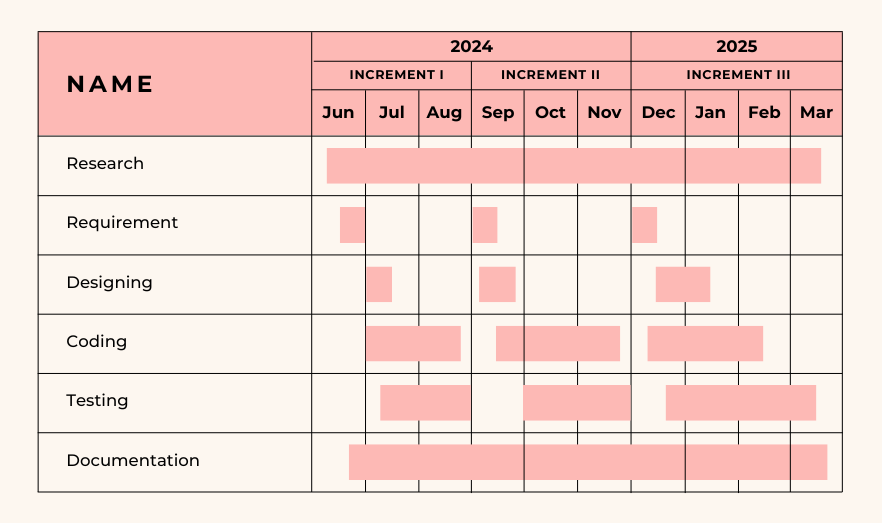
\includegraphics[scale=0.5]{images/gantt.png}
    \caption{Gantt Chart}
\end{figure}

The team's project was initially on Topic modelling of Resumes and Job Descriptions. Job Descriptions can be scraped through a popular site 'Indeed'. However, the resumes on 'Hireitpeople' were deemed unsufficient. Our objective was to have a topic model that can provide topic distribution for resumes and job descritions. To cover all jobs in recent time is a job of large scale, so the focus was on technical jobs. Job Descriptions, for each job scraped around thousand documents, were ready. Resume for Software Engineers, Network administrators, Web Developer, Project Manager, Database Administrators and Security Analyst are widely available, but unfortunately other jobs such as technical support specialists, video game developers are scarce on the internet. The option of scraping Linkedin is problematic as it requires login session, and Linkedin have a rate limit of searching and viewing profile(80 per day) on new account and accounts with limited connectivity. Another option which, would be best if possible, was ProxyCurl. ProxyCurl manages huge database of linkedin profile, and provides its data through API(Application Programming Interface) for commercial use. This means that each profile scrap costs \$0.020, and for our scale i.e 40000 resumes for 40 technical jobs could cost well over \$800. This predicament led to change of our Project.


\chapter{Litreature Review}

\section{Related Work}
The paper “Nepali Offensive Language Detection Using Transfer Learning Techniques” \cite{suwal2023nepali} explores offensive language detection and sentiment classification in Nepali text using pre-trained models like XLM-RoBERTa, BERT, NepBERTa, and distilBERT-base-Nepali. For Named Entity Recognition (NER), distilBERT-base-Nepali achieved 36.77\% F1-score with 85.67\% accuracy, while deberta-base-Nepali reached an F1-score of 40.14\% and 86.6\% accuracy. In sentiment analysis, distilBERT-base-Nepali excelled with a 72.24\% accuracy and 71.8\% F1-score. However, since the NepSA dataset was created for aspect term extraction, and Sentiment classification, even with balanced dataset, has duplicate Text for a Class with Same or different class Polarity. This arises the question of data leakage while training the models which in turn leads to optimistic performance. This issue is addressed in our project by cleaning such instances.

Paper, "Named-entity based sentiment analysis of Nepali news media texts", scrapped text data from Nepali news medias: Kantipur Daily, NagarikNews, Online Khabar and Setopati, maintaining dataset with 2676 positive instance and  814 negative \cite{shrestha2020named}. Classification was done by balancing each class to 814, which saw F1- score of 80.2 using SVM. The experimentation was done on SVM, Random Forrest and Decision Tree, while the embeddings for these classifiers were generated by testing Word2Vec and FastText.

Hate speech and abusive language have become a common phenomenon on Arabic social media. Automatic hate speech and abusive detection systems can facilitate the prohibition of toxic textual contents. The complexity, informality, and ambiguity of the Arabic dialects hindered the provision of the needed resources for Arabic abusive/hate speech detection research. The paper, "L-hsab: A levantine twitter dataset for hate speech and abusive language" introduces the first publicly-available Levantine Hate Speech and Abusive (L-HSAB) Twitter dataset with Krippen-dorff’s /alpha value 76.5\% \cite{mulki2019hsab}. The dataset consists of 5,846 tweets, labeled as Hate, Abusive, or Normal. To ensure a reliable annotation process, the authors provided clear guidelines, inter-annotator agreement metrics, and conducted evaluations to establish the dataset's consistency. Machine learning classifiers such as Naive Bayes and SVM were tested, with Naive Bayes achieving better results in both binary and multi-class classification tasks. Naive Bayes from NLTK achieved an average of 82\% F1-score among Hate and Abusive class. Both classifiers were trained with several n-gram schemes with Term frequency weighting. 

In their 2022 study, Maskey et al. conducted a comparative analysis of Transformer-based language models for Nepali text classification, focusing on DistilBERT, DeBERTa, and XLM-RoBERTa. The research aimed to identify effective strategies for pre-training and fine-tuning these models within the context of a low-resource language. The models were evaluated on a downstream classification task using the "16 Nepali News" dataset, which comprises approximately 14,364 news documents categorized into 16 distinct groups.
The findings revealed that all models surpassed the baseline accuracy of 80\%. DeBERTa achieved the highest accuracy at 88.93\%, highlighting the significance of training domain-adapted language models. DistilBERT attained a respectable accuracy of 88.31\% with the least number of training steps, implying faster training for downstream tasks. The marginal performance difference compared to DeBERTa, combined with its smaller and lighter architecture, makes DistilBERT particularly well-suited for deployment in production environments with computational constraints. This study underscores the potential of leveraging efficient Transformer models like DistilBERT for low-resource languages, providing a foundation for future NLP research and applications in Nepali.

\chapter{Methodology}

\section{Working Mechanism}

\begin{figure}[h]
\centering
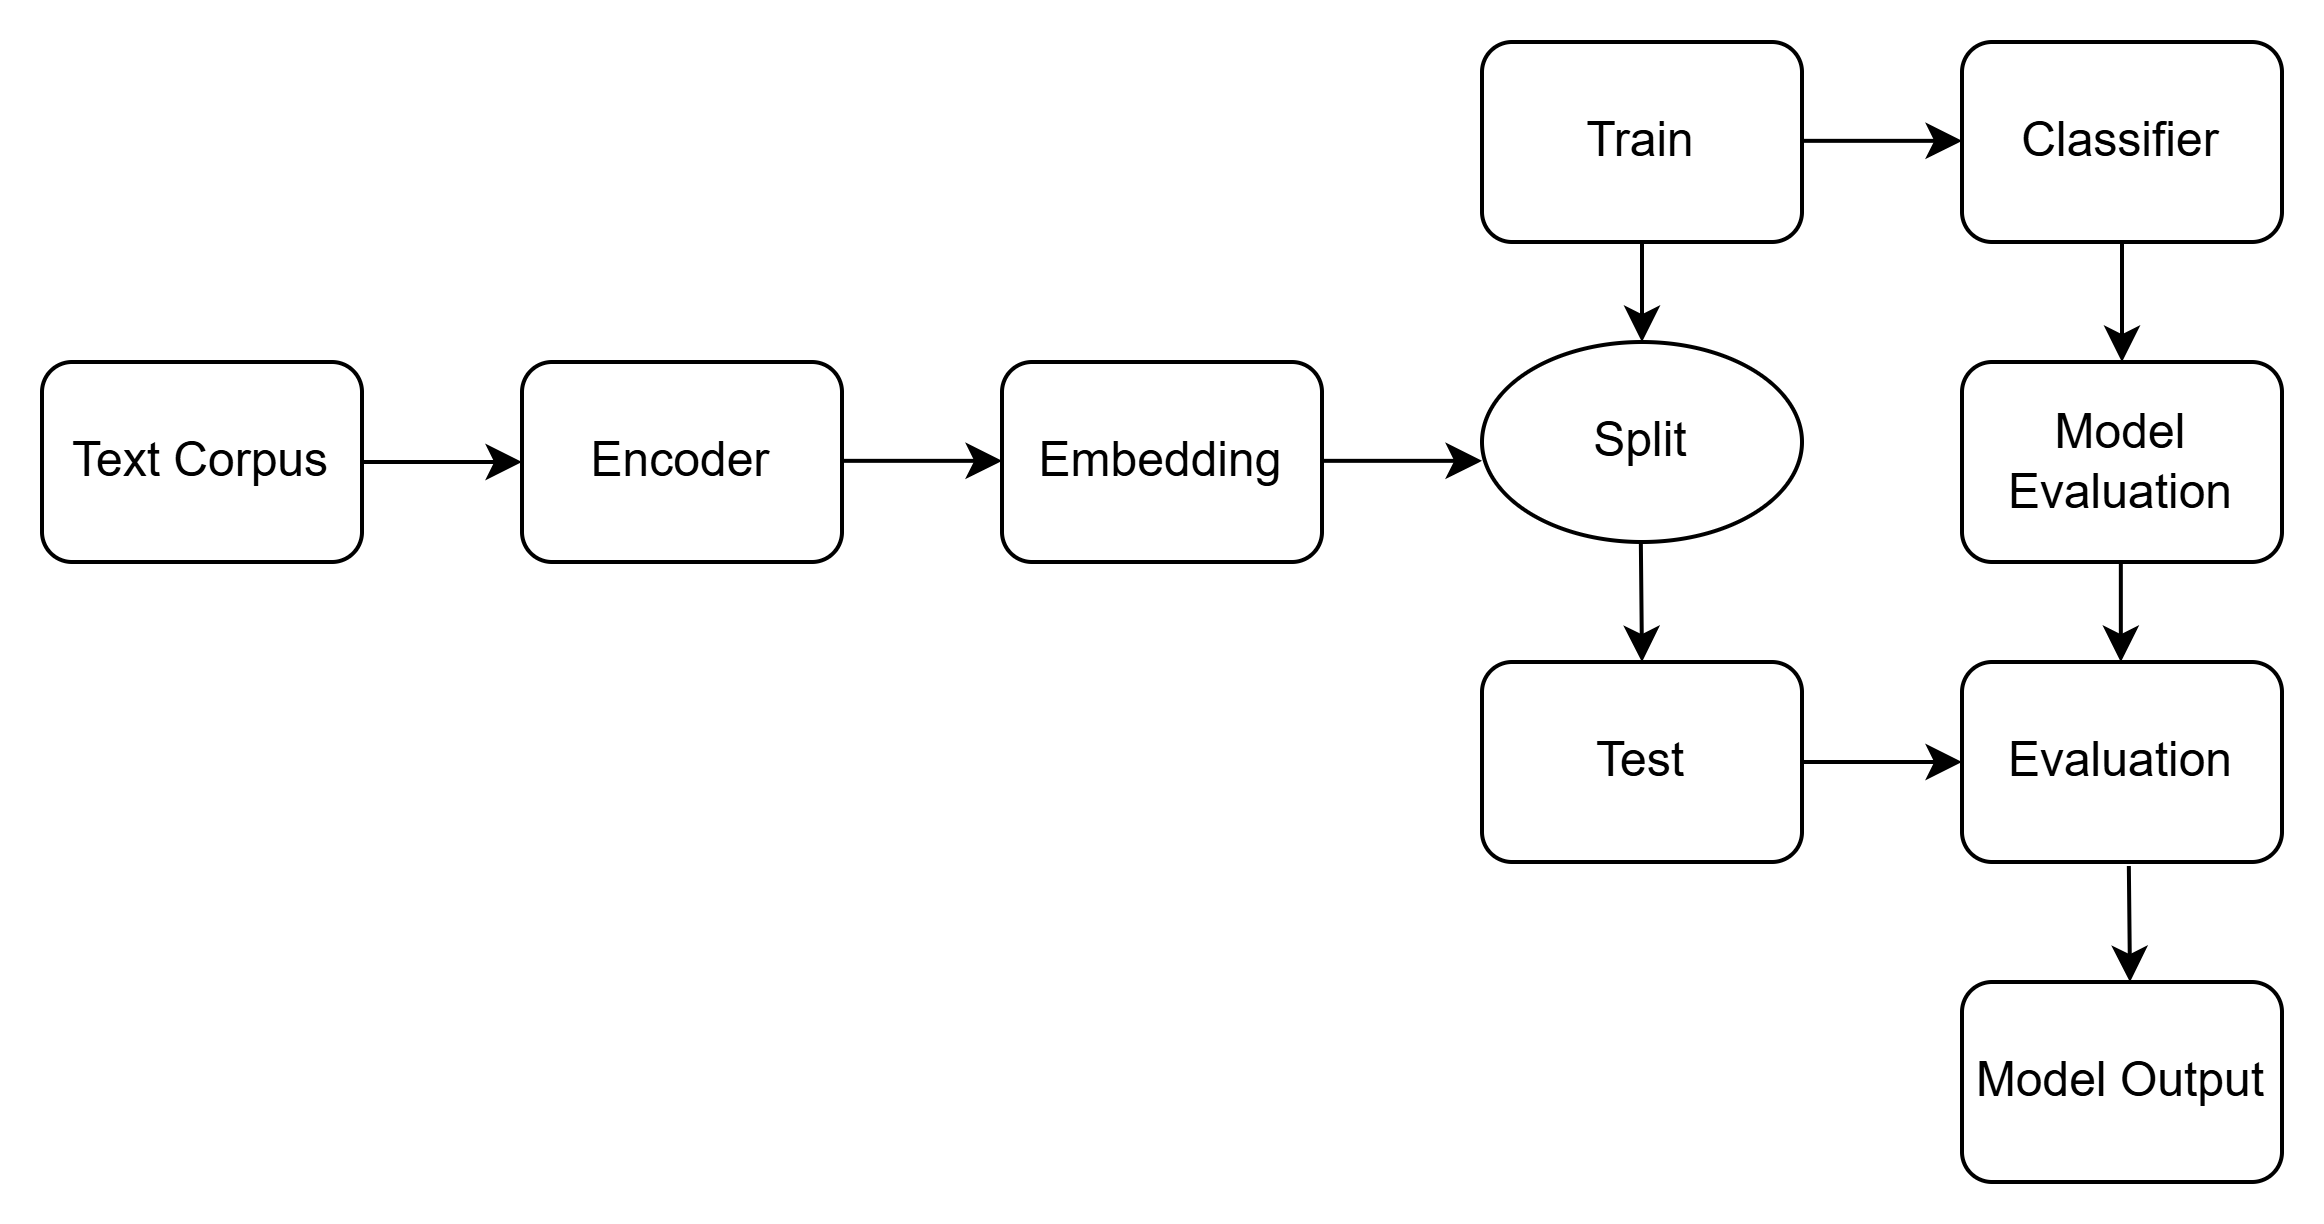
\includegraphics[scale=0.23]{images/methodology.png}
\caption{Block diagram of Working Mechanism}
\end{figure}
The proposed structure of the project includes different steps. The texts for sentiment classification after preprocessing are embedded into feature vectors through the usage of popular encoders such as Word2Vec. These encoded features are then split into Train and test set at the ratio of 7:3.
\subsection{Data Collection}
The Nepali Sentiment Analysis (NepSA) dataset serves as the foundation for our project, providing valuable insights into abusive content in the Nepali language. This dataset was specifically chosen for its unique features, which addresses the complex linguistic challenges associated with abusive language detection in Nepali \cite{singh2020aspect}.
The dataset was compiled from comments collected from popular Nepali YouTube channels, primarily within the News and Politics category, focusing on channels with the highest subscriber base. It consists of 3,068 comments extracted from 37 videos across 9 distinct channels. The dataset follows a binary sentiment polarity framework, categorizing comments into key aspects: General, Profanity, Violence. The total count of instances in the dataset account to 3529. Each comment is annotated based on the sentiment expressed towards a specific target entity, enabling a more detailed and context-specific understanding of the language rather than a generalized sentiment analysis.
\begin{figure}[h]
\centering
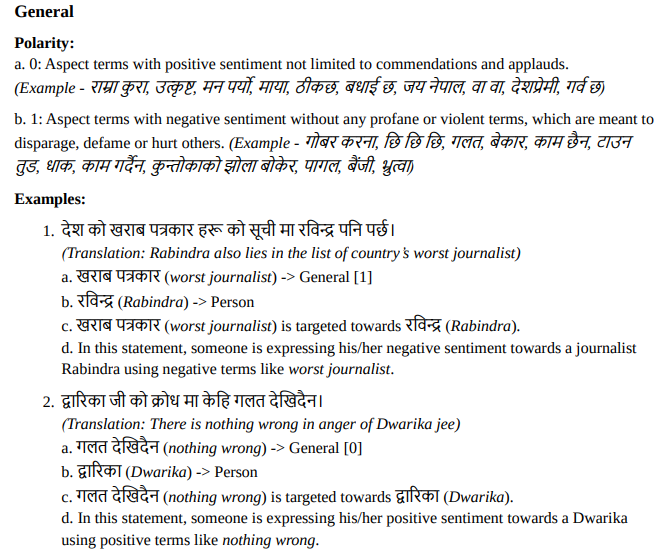
\includegraphics[scale=0.65]{images/1.png}
\caption{Class example 1}
\end{figure}

\newpage

\begin{figure}[h]
\centering
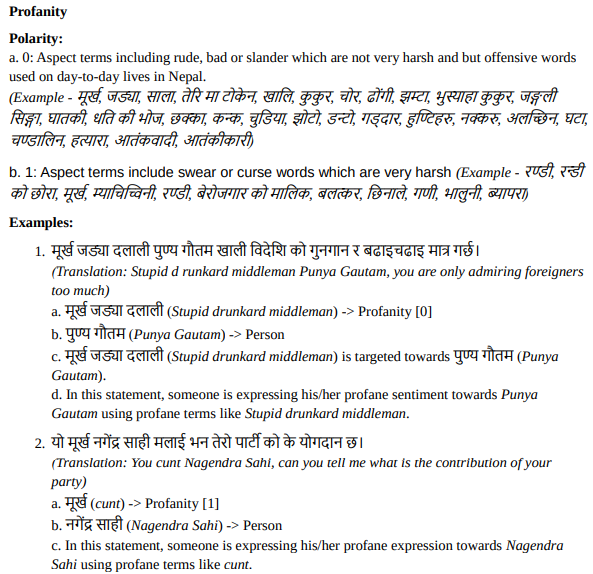
\includegraphics[scale=0.65]{images/2.png}
\caption{Class example 2}
\end{figure}

\newpage

\begin{figure}[h]
\centering
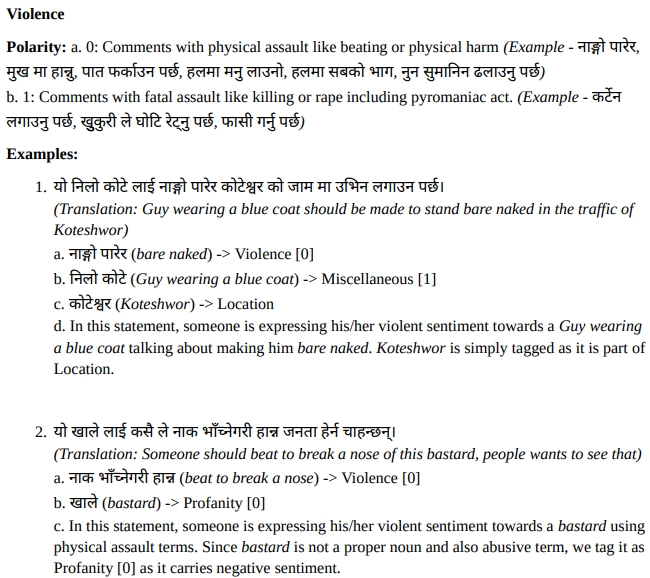
\includegraphics[scale=0.65]{images/3.png}
\caption{Class example 3}
\end{figure}

\newpage


\subsection{Data Preprocessing}
The process of pre-processing the data is very important as good data is very important for effective learning by Classifiers.

\begin{figure}[h]
\centering
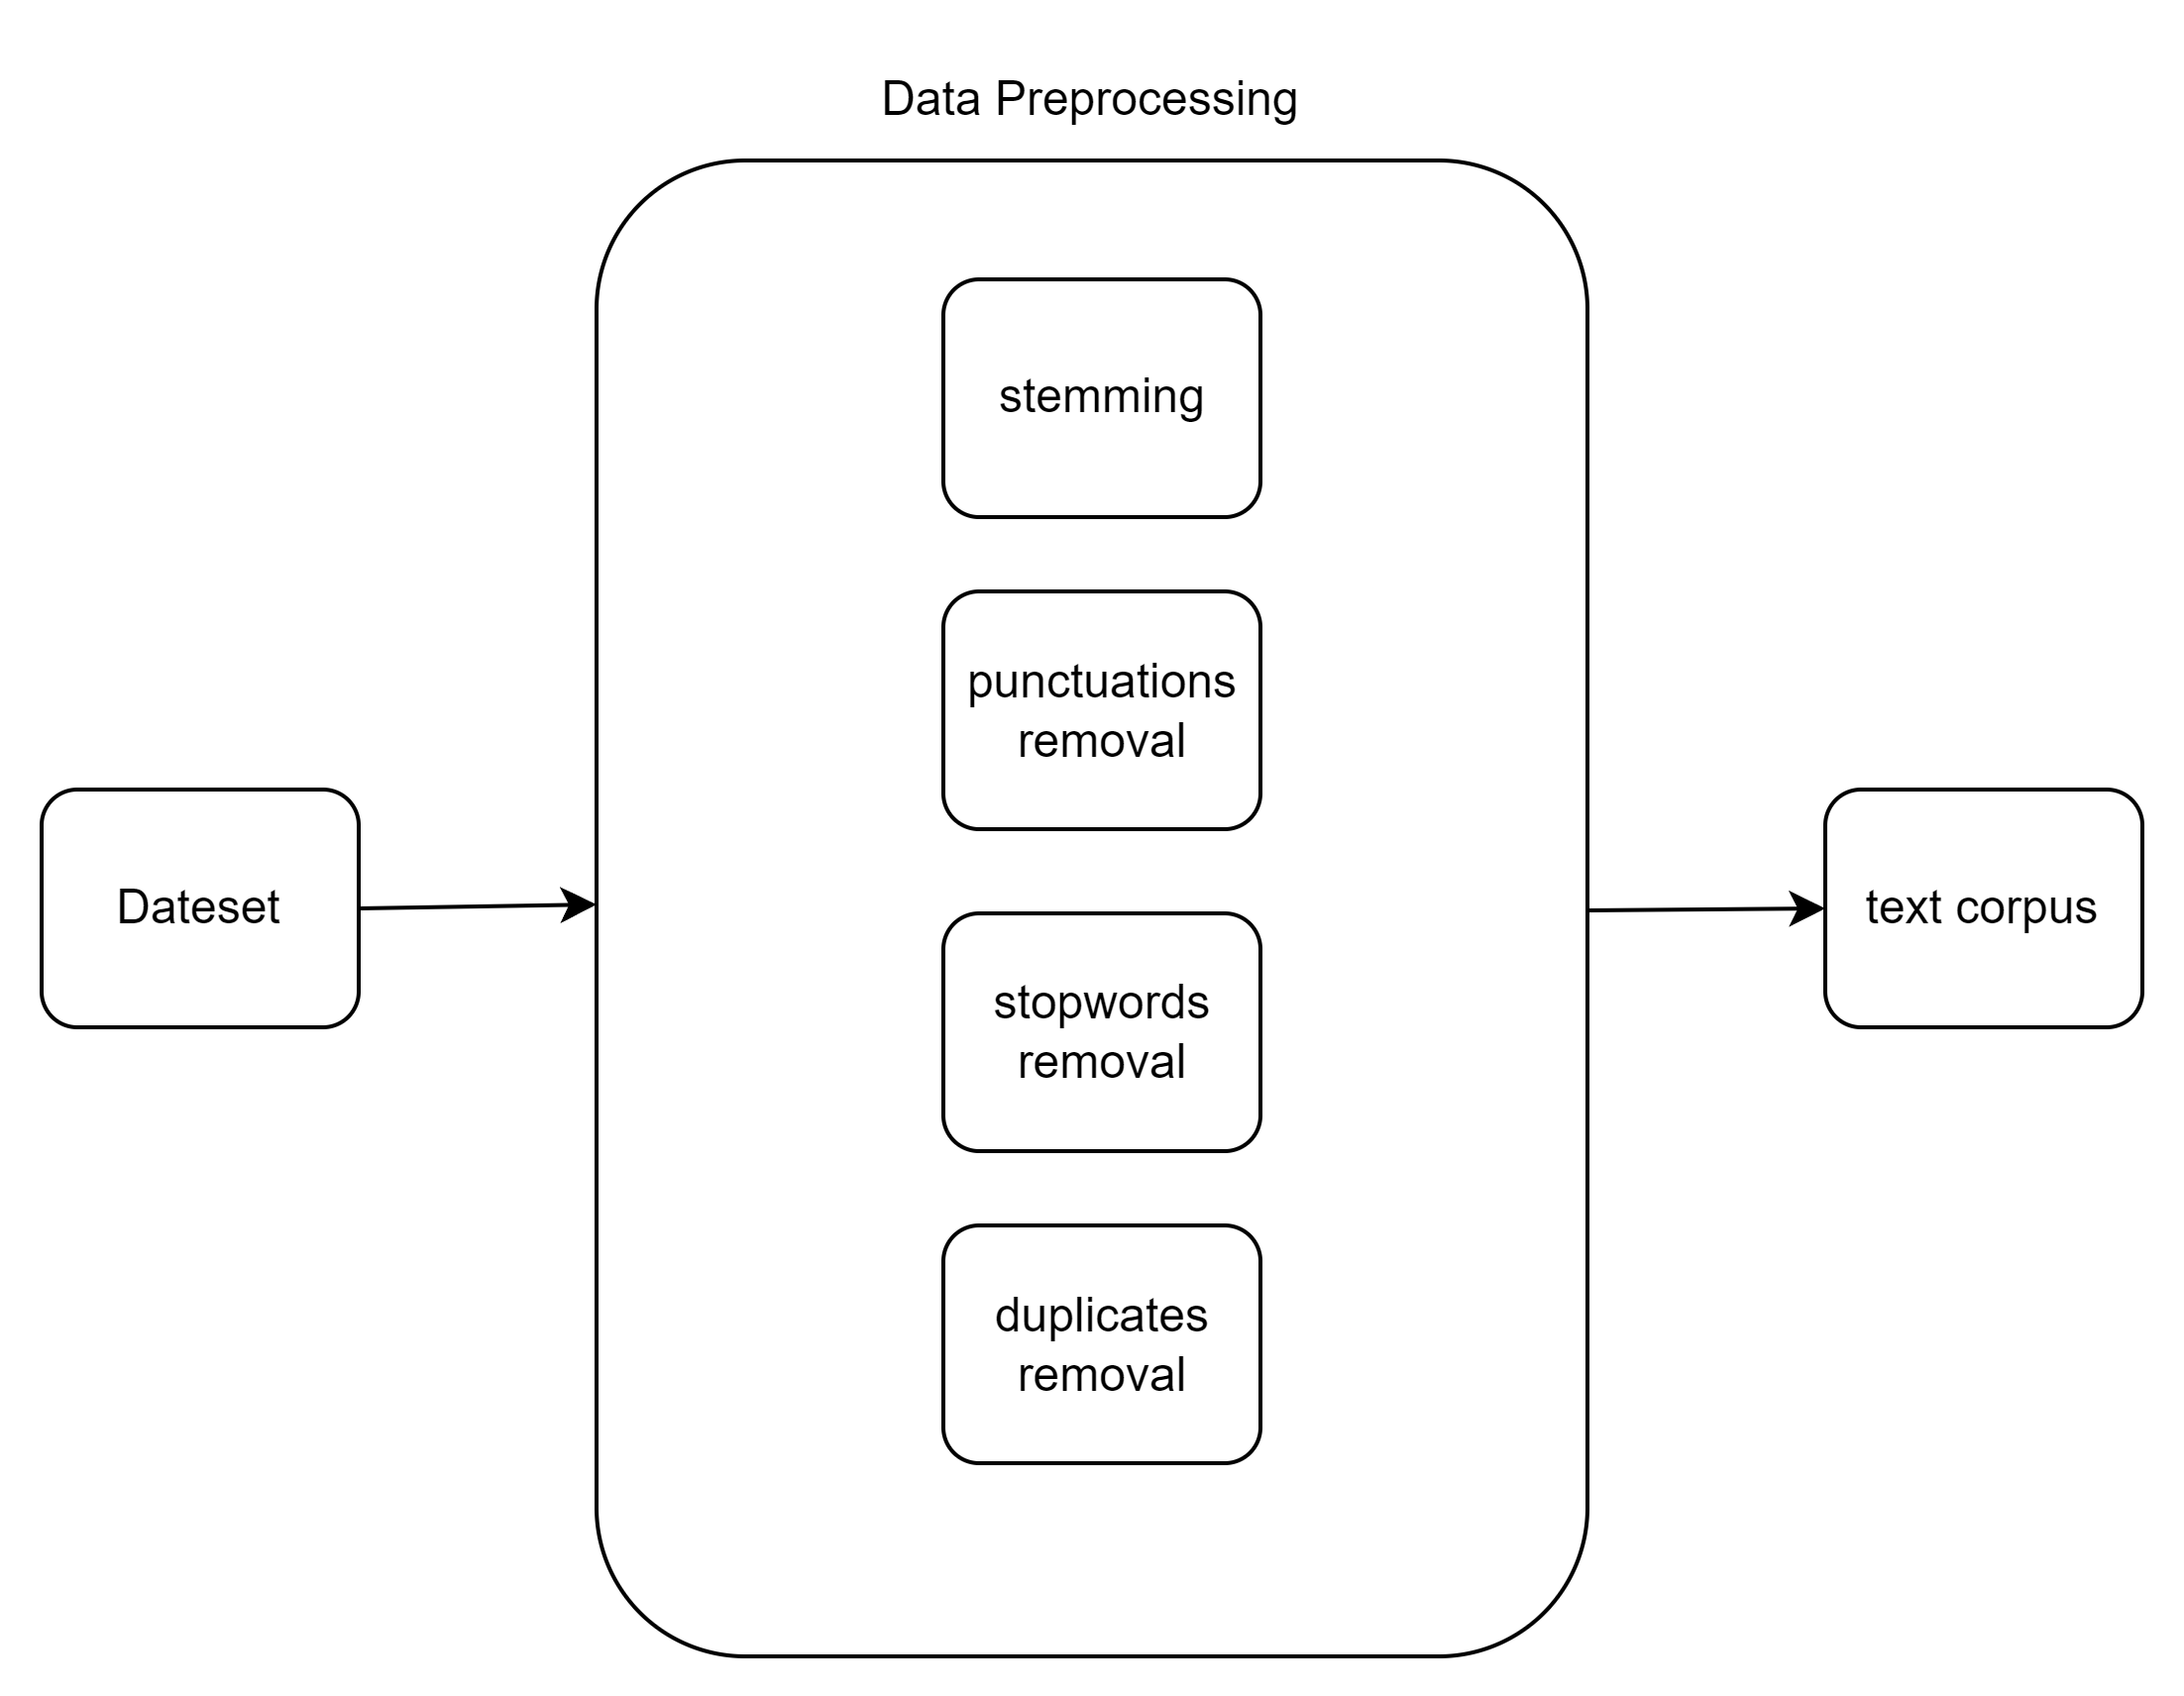
\includegraphics[scale=0.2]{images/meth.png}
\caption{Block diagram of Data Preprocessing}
\end{figure}

The dataset was prepared using Nepali Stemmer.Furthermore, the punctuations in texts were removed followed by stopwords removal using NLTK stopwords package. Since, the dataset was created with priority on aspect term extraction there are instances of same text classified as duplicates with different Aspect(in same class, and different class). These duplicates, in class with higher count, was removed to have unique instances for training and avoid data leakage. By removing such duplicates the data instances amount to 2859.\\
Inorder to classify among textual multi-classes: "GENERAL", "VIOLENCE" and "PROFANITY", label encoding is done.
\subsection{Machine Learning Techniques}
\subsubsection{Support Vector Machine(SVM)}
Support Vector Machine (SVM) constructs a hyperplane or set of hyperplanes in a high- or infinite-dimensional space, which can be used for classification, regression, or other tasks. The Support Vector Machine (SVM) stands as a supervised machine learning algorithm with applications in both classification and regression tasks. While SVM is versatile enough to handle regression problems, its optimal utility lies in the domain of classification. The central objective of the SVM algorithm involves the identification of a hyperplane within an N-dimensional space that distinctly segregates the data points. The dimensionality of this hyperplane is contingent upon the quantity of input features.\\
In the context of hate speech detection, the SVM algorithm aims to segregate hate speech from non-hate speech based on features extracted from the text. For two input features, the hyperplane is represented as a line, while for three input features, it assumes the form of a 2-dimensional plane. As the number of features increases, the hyperplanes become increasingly complex and multidimensional, enabling precise classification even in high-dimensional feature spaces \cite{pralhad}.
\begin{figure}[h]
\centering
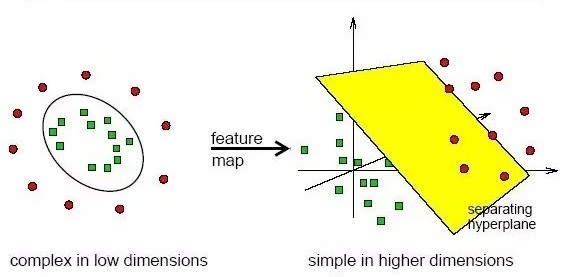
\includegraphics[scale=0.65]{images/svm.png}
\caption{SVM}
\textit{Source:https://www.dtreg.com/solution/support-vector-machines}
\end{figure}

\subsection{Word2Vec}
Word2Vec is a neural network-based algorithm used to generate vector representations of words, capturing their semantic relationships within a text corpus. Word2Vec maps words into a continuous vector space where semantically similar words are positioned closer together. This results in dense word embeddings that effectively represent both syntactic and semantic properties of words.

\subsubsection{Working Mechanism of Word2Vec}
Word2Vec operates using two primary architectures: Continuous Bag of Words (CBOW) and Skip-Gram.
\begin{itemize}
\item CBOW predicts a target word based on its surrounding context words. For example, in the sentence ``The cat sat on the \_\_\_," the model predicts the missing word ``mat" using the words around it. This method is efficient for larger datasets and captures general word associations.
\item Skip-Gram works inversely, predicting the context words around a given target word. For example, given the word ``cat," the model predicts surrounding words like ``the" or ``sat." Skip-Gram is particularly effective for learning embeddings for rare words, as it focuses on the word's relationships in specific contexts.
\end{itemize}

Both architectures use a shallow neural networks to optimize the word embeddings. Through training, the model minimizes the error in predictions, adjusting the word vectors to reflect their contextual similarities and differences. This results in embeddings where words with similar meanings or usage patterns are positioned closer together in the vector space.
In this project, Word2Vec is used to generate embeddings for Nepali text, enabling the detection of abusive and offensive language within specific contexts. By understanding the relationships between words such as `thief' or `dog' (in nepali text), the algorithm allows the system to identify clusters of abusive terms and interpret them based on their context. This enhances the accuracy and robustness of the hate speech detection model.

For embedding generation, we employed a pre-trained Word2Vec model which has 300-dimensional vectors for more than 0.5 million Nepali words and phrases \cite{dz6s-my90-19} on CBOW architecture. This model was fine-tuned with our text corpus.
\subsection{TF-IDF Formula}
TF-IDF is a statistical measure that quantifies the importance of words in a document relative to a collection (corpus) of documents. It reflects how relevant a term is to a document by balancing two metrics: Term Frequency (TF) and Inverse Document Frequency (IDF).
\begin{enumerate}
    \item \textbf{Term Frequency (TF):}
    \[
    TF(t, d) = \frac{\text{Number of occurrences of term } t \text{ in document } d}{\text{Total number of terms in document } d}
    \]

    \item \textbf{Inverse Document Frequency (IDF):}
    \[
    IDF(t) = \log \left( \frac{\text{Total number of documents}}{\text{Number of documents containing term } t} + 1 \right)
    \]

    \item \textbf{TF-IDF Score:}
    \[
    TF\text{-}IDF(t, d) = TF(t, d) \times IDF(t)
    \]
\end{enumerate}

\subsection{NepBERTa and Its Working Mechanism}
NepBERTa is a specialized pre-trained language model for the Nepali language based on the robust BERT (Bidirectional Encoder Representations from Transformers) architecture. It uses deep learning to produce word embeddings tailored specifically to the linguistic nuances of Nepali. Unlike traditional models, NepBERTa understands the context of a word in all directions (left and right of the word), allowing it to generate more accurate and nuanced embeddings for Nepali text.

\subsubsection{Steps for NepBERTa}
\textbf{Step 1: Tokenization}\\
The input Nepali text is tokenized into a sequence of tokens,\begin{equation}
x = [x_1, x_2,......, x_n]
\end{equation}
using a WordPiece tokenizer customized for the Nepali language. This ensures that the model can efficiently handle Nepali-specific words and subwords.\\
\textbf{Step 2: Embeddings}\\
Each token is mapped to a dense vector space using a learned embedding matrix \textbf{E}. The embedding for each token is the sum of three components:
\begin{equation}
e_i = E(x_i) + E_{seg}(x_i) + E_{pos}(i)
\end{equation}
Where:\begin{itemize}
\item \(E_{seg}(x_i)\): Segment embedding, indicating whether the token belongs to the first or second segment (e.g., sentence A or sentence B).
\item \( E_{pos}(i)\): Position embedding, representing the token's position in the sequence.
\end{itemize}
\textbf{Step 3: Encoder}\\
The embedded tokens are passed through a multi-layer bidirectional Transformer encoder, consisting of L identical layers. Each layer applies self-attention and a feed-forward neural network (FFNN):
\begin{equation}
h^l = \text{TransformerLayer}(h^{l-1})
\end{equation}
Where:
\begin{itemize}
    \item \( h^l \): The output of the \( l \)-th layer.
    \item \( h^0 \): The embedding input.
\end{itemize}
\textbf{Step 4: Pooling}
The final output of the encoder, \( h^L \), is a sequence of vectors. The first vector, \( h^L[0] \), is used as the overall representation of the input sequence:
\begin{equation}
p = h^L[0]
\end{equation}
\textbf{Step 5: Pre-training Tasks}\\
NepBERTa is pre-trained using Masked Language Modeling (MLM), where random tokens in the Nepali text are masked, and the model learns to predict the original tokens based on the context. The MLM loss is defined as:
\begin{equation}
L_{\text{mlm}} = -\sum x_i \log\big(p(x_i \mid x_{-i})\big)
\end{equation}

\subsection{DistilBERT and its Key Methodologies}
DistilBERT is a streamlined version of the BERT (Bidirectional Encoder Representations from Transformers) model, designed to enhance efficiency in natural language processing tasks. It reduces BERT’s size by 40\%, offers 60\% faster inference, and is 71\% faster on mobile applications. Despite being compact, it retains 97\% of BERT’s accuracy, making it an effective alternative to BERT. It achieves this through several key methodologies:
\subsubsection{Knowledge Distillation}
Knowledge distillation is a model compression technique where a smaller model (the student) is trained to replicate the behavior of a larger, pre-trained model (the teacher). In the case of DistilBERT, the BERT model serves as the teacher. The student model learns to predict the output probabilities of the teacher, capturing the nuanced information learned by the larger model. This process enables the student model to achieve high performance with reduced complexity.

\subsubsection{Loss Functions in DistilBERT}
\begin{enumerate}
    \item \textbf{Distillation Loss (KL Divergence Loss)}
    Distillation hello  loss is essential in training the student model during knowledge distillation. It's calculated by comparing the student's prediction probability to the soft probabilities provided by the teacher model. The soft probabilities for the student model are computed as:\\
    \[
(y_S^T)_i = \frac{\exp((z_S)_i/T)}{\sum_j \exp((z_S)_j/T)}
\]
    The distillation loss is then calculated as:\\
    \[
\mathcal{L}_{KD} = \alpha T^2 * \mathcal{L}_{CE}(y_T^T, y_S^T) + (1 - \alpha) * \mathcal{L}_{CE}(y_S, y_{true})
\]

where:
\textbf{temperature T} smooths the probability distribution, making it easier for the student model to learn
 	L(CE)  KL divergence is used as the loss function to measure the difference between the teacher’s and student’s probability distributions.
\item \textbf{Masked Language Modeling (MLM) Loss}\\
Like BERT, DistilBERT learns language patterns using masked language modeling (MLM). In this approach, some words in a sentence are randomly replaced with a special token, and the model predicts these masked words based on surrounding context. The loss is computed as:\\
\[
\mathcal{L}_{MLM} = \sum -y_{true} \log(y_S)
\]

\item \textbf{Cosine embedding loss}
Cosine embedding loss helps the student model match the teacher model’s embeddings by minimizing their cosine distance, preserving knowledge while reducing model size. Cosine similarity is defined as:\\
\[
\cos(\mathbf{x_1}, \mathbf{x_2}) = \frac{\mathbf{x_1} \cdot \mathbf{x_2}}{\|\mathbf{x_1}\| \|\mathbf{x_2}\|}
\]
The Cosine embedding loss is computed as:
\[
\mathcal{L}_{cos}(\mathbf{x_1}, \mathbf{x_2}) = 1 - \cos(\mathbf{x_1}, \mathbf{x_2})
\]
To effectively train the student model, DistilBERT employs a triple loss function that combines Distillation loss, MLM loss and Cosine embedding loss. The final training loss function is a weighted sum of the three loss components:\\
\[
\mathcal{L} = \alpha_d T^2 * \mathcal{L}_{dist} + \alpha_{mlm} * \mathcal{L}_{MLM} + \alpha_{cos} * \mathcal{L}_{cos}
\]

The following hyperparameter values were used during the training of DistilBERT:\\
Temperature (T) = 2.0\\
Distillation weight () = 5.0\\
MLM loss weight () = 2.0\\
Cosine loss weight () = 1\\


\end{enumerate}

\subsection{DistilBERT Architecture}
DistilBERT reduces the number of layers to 6 from 12 in the original BERT architecture, resulting in a model with 66M parameters. This reduction leads to a 60\% increase in inference speed while maintaining approximately 97\% of BERT's language understanding capabilities.\\



In the context of developing efficient natural language processing models for the Nepali language, DistilBERT emerges as a compelling choice due to its reduced model size and computational efficiency. A study titled "Nepali Encoder Transformers: An Analysis of Auto Encoding Transformer Language Models for Nepali Text Classification" highlights the advantages of using smaller transformer models like DistilBERT. The research emphasizes that such models are particularly beneficial for low-resource languages like Nepali, where computational resources may be limited. By employing DistilBERT, which maintains a balance between performance and efficiency, it becomes feasible to develop robust language models without the need for extensive computational infrastructure.


\subsubsection{Architecture Modification}
DistilBERT reduces the number of layers in the original BERT architecture by half, resulting in a model with 40\% fewer parameters. This reduction leads to a 60\% increase in inference speed while maintaining approximately 97\% of BERT's language understanding capabilities. The streamlined architecture makes DistilBERT more suitable for deployment in resource-constrained environments.
In the context of developing efficient natural language processing models for the Nepali language, DistilBERT emerges as a compelling choice due to its reduced model size and computational efficiency. A study titled "Nepali Encoder Transformers: An Analysis of Auto Encoding Transformer Language Models for Nepali Text Classification" highlights the advantages of using smaller transformer models like DistilBERT. The research emphasizes that such models are particularly beneficial for low-resource languages like Nepali, where computational resources may be limited. By employing DistilBERT, which maintains a balance between performance and efficiency, it becomes feasible to develop robust language models without the need for extensive computational infrastructure.

\subsubsection{Condensed Nearest Neighbour (CNN)}
Condensed Nearest Neighbour (CNN) is a data reduction technique used to improve the efficiency of classification tasks, especially in small datasets. It works by selecting only the most informative samples that define decision boundaries, ensuring misclassified instances are retained while redundant data is removed. This makes CNN effective in simplifying datasets, reducing noise, and enhancing model performance without losing critical information.

\subsubsection{Neighbourhood Cleaning Rule (NCR)}
Neighbourhood Cleaning Rule (NCR) is an undersampling technique used to improve dataset quality by focusing on removing noisy or ambiguous samples. It works by identifying majority-class samples that are either misclassified by their nearest neighbours or surrounded by minority-class neighbours. These samples are removed, resulting in a cleaner and more balanced dataset. NCR is particularly useful for small datasets as it retains critical decision boundaries while reducing noise and ambiguity, improving the overall performance of classification models.

\subsubsection{Random Under Sampler}
Random Under Sampler is a simple undersampling technique used to handle class imbalance in datasets. It works by randomly removing samples from the majority class until its size matches the minority class. This helps balance the dataset and prevents the model from being biased toward the majority class. While it is fast and easy to implement, it can potentially remove important data points. It is most suitable when working with small datasets, as it reduces size without requiring extensive computational resources.

\subsubsection{SMOTE (Synthetic Minority Oversampling Technique)}
SMOTE is an oversampling method used to address class imbalance in datasets by generating synthetic samples for the minority class. It works by selecting a sample from the minority class and creating new synthetic data points by interpolating between that sample and one of its nearest neighbours. This process helps balance the dataset without simply duplicating existing samples. SMOTE is effective in improving model performance, especially for small datasets, as it enhances representation of the minority class while preserving the overall data distribution.

\subsubsection{ADASYN (Adaptive Synthetic Sampling)}
ADASYN is an advanced oversampling technique that generates synthetic samples for the minority class, focusing more on harder-to-classify instances. It works by identifying samples in the minority class that are difficult to classify (i.e., surrounded by majority-class neighbours) and generating more synthetic data for these instances. This adaptive approach ensures better balance while improving decision boundaries for the minority class. ADASYN is particularly effective in small datasets with complex class distributions, as it reduces bias and enhances model performance in imbalanced datasets.

\section{SONAR(Sentence-Level Multimodal and Language-Agnostic Representations )}
SONAR, developed by Facebook Research, is a multilingual and multimodal embedding model that provides fixed-size representations for both text and speech.
SONAR leverages deep learning architectures to generate embeddings that capture semantic relationships between words and sentences. The model supports over 200 languages, making it effective for low-resource languages like Nepali.
Unlike traditional techniques like TF-IDF and Word2Vec, SONAR embeddings retain word meanings based on context.
Text from different languages is embedded into a common space, allowing cross-lingual transfer.
\subsection{Why over other models }
SONAR outperforms LASER3 and LaBSE on xsim and xsim++ similarity search tasks.
 Unlike models like BERT and XLM-R, which provide variable-length representations, SONAR produces consistent 1024-dimensional embeddings.
\subsection{How SONAR Works}
SONAR transforms text and speech into embeddings using a Transformer-based encoder-decoder model. The process follows:
\subsection{Sentence Tokenization}
Given a sentence $S$ consisting of words:
\begin{equation}
    S = \{w_1, w_2, \dots, w_n\}
\end{equation}

\subsection{Encoding Function}
SONAR applies a function $f$ to transform the sequence into a fixed-size vector:
\begin{equation}
    E(S) = f(w_1, w_2, \dots, w_n)
\end{equation}
where $E(S)$ is a 1024-dimensional embedding vector.

\subsection{Training Objectives}
SONAR is trained using multiple loss functions:
\begin{itemize}
    \item \textbf{Translation Loss} ($L_{MT}$): Ensures that sentence embeddings are effective for translation tasks.
    \item \textbf{Mean Squared Error Loss} ($L_{MSE}$): Aligns embeddings of different languages.
    \item \textbf{Denoising Auto-Encoding Loss} ($L_{DAE}$): Improves robustness by reconstructing noisy inputs.
\end{itemize}
The final training objective combines these:
\begin{equation}
    L = L_{MT} + \alpha \cdot L_{MSE} + \beta \cdot L_{AE/DAE}
\end{equation}

\section{SONAR Architecture}
SONAR follows a two-step training process:

\subsection{Multilingual Text Sentence Embedding Space}
\begin{itemize}
    \item Uses an encoder-decoder Transformer model.
    \item Pretrained using the NLLB 1B model.
    \item Embeddings are generated through mean-pooling on token-level outputs.
\end{itemize}

\subsection{Speech Sentence Embedding Space (Teacher-Student Approach)}
\begin{itemize}
    \item A speech encoder is trained to match text embeddings.
    \item Uses pre-trained w2v-BERT for initialization.
    \item Speech embeddings are mapped to the same 1024-dimensional space.
\end{itemize}

\section{Differential Evolution}
Differential evolution is a stochastic population-based method that is useful for global optimization problems. At each pass through the population, the algorithm mutates each candidate solution by mixing with other candidate solutions to create a trial candidate. There are several strategies for creating trial candidates, which suit some problems more than others.\\
The 'best1bin' strategy is a good starting point binomial distribution. In this strategy, two members of the population are randomly chosen. Their difference is used to mutate the best member (the ‘best’ in ‘best1bin’), $x_0$, so far:
\begin{equation}
    b' = x_0 + F \cdot (x_{r0} - x_{r1})
\end{equation}
where, $F$ is the \textit{mutation} parameter, \(x_0\) is the base vector, \(x_{r0}\) and \(x_{r1}\) are two randomly selected vectors from the population. A trial vector is then constructed. Starting with a randomly chosen $i$th parameter, the trial is sequentially filled (in modulo) with parameters from $b'$ or the original candidate. The choice of whether to use $b'$ or the original candidate is made with a binomial distribution (the ‘bin’ in ‘best1bin’) - a random number in $[0,1]$ is generated. If this number is less than the \textit{recombination} constant, then the parameter is loaded from $b'$, otherwise, it is loaded from the original candidate. The final parameter is always loaded from $b'$.\\
Once the trial candidate is built, its fitness is assessed. If the trial is better than the original candidate, then it takes its place. If it is also better than the best overall candidate, it also replaces that.

\subsection{Parameters of Differential Evolution}
\begin{enumerate}
\item \textbf{func : callable}\\
The objective function to be minimized. Must be in the form f(x, *args), where x is the argument in the form of a 1-D array and args is a tuple of any additional fixed parameters needed to completely specify the function.
\item \textbf{bounds : sequence}\\
Bounds for variables. (min, max) pairs for each element in x, defining the lower and upper bounds for the optimizing argument of func. It is required to have len(bounds) == len(x). len(bounds) is used to determine the number of parameters in x.
\item \textbf{maxiter : int, optional}\\
The maximum number of generations over which the entire population is evolved. The maximum number of function evaluations (with no polishing) is:\\ \((maxiter + 1) * popsize * len(x)\)

\item \textbf{tol : float, optional}\\
Relative tolerance for convergence, the solving stops when\\ \(np.std(pop) <= atol + tol * np.abs(np.mean(population\_energies))\), where atol and tol are the absolute and relative tolerance respectively.

\item \textbf{mutation : float or tuple}\\
The mutation constant. In the literature this is also known as differential weight, being denoted by F. If specified as a float it should be in the range [0, 2]. If specified as a tuple (min, max) dithering is employed. Dithering randomly changes the mutation constant on a generation by generation basis. The mutation constant for that generation is taken from U[min, max). Dithering can help speed convergence significantly. Increasing the mutation constant increases the search radius, but will slow down convergence.

\item \textbf{recombination : float, optional}\\
The recombination constant, should be in the range [0, 1]. Increasing this value allows a larger number of mutants to progress into the next generation, but at the risk of population stability.
\end{enumerate}

Optuna \cite{optuna_2019} is a software framework used for automating optimization process of hyperparameters. By trial and error process,it automatically searches for and finds the optimal hyperparameter values for excellent performance.
It uses a history record of trials inorder to determine which hyperparameter values to try next. Using this data, it estimates a promising area and tries values in that area. Optuna repeats this process using the history data of trials that are completed so far. It employs a Bayesian optimization algorithm called Tree-structured Parzen Estimator \cite{tree_structured}.
It uses Pruning algorithm which in general works in two phases.
\begin{enumerate}
\item It periodically monitors the intermediate objective values
\item It terminates the trial that does not meet the predefined condition.
\end{enumerate}


\section{Development Model}
The Incremental model, which is a mixture of waterfall and iterative development approach is opted, as the project demands few requirements and is fairly simple. As the name suggests, the major objective is focused as the first increment of the project. The activities in this model are completed iteratively and each outcome acts as an input for the next phase, thus increments are developed in such a way.
\begin{figure}[h]
	\centering
	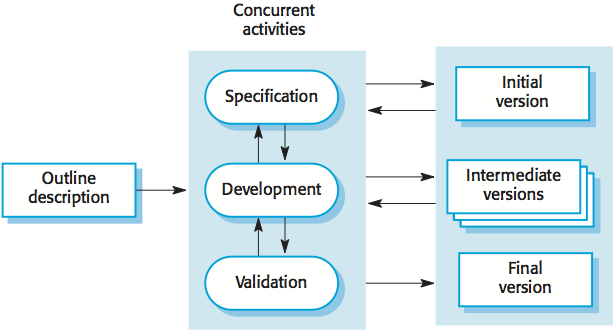
\includegraphics[scale=1.3]{incremental.png}
	\caption{Development Model}
\end{figure}
\subsection{Requirement Specification}
The project requires an optimized model that can effectively classify among different class types while learning the context in texts. Finally, the model is interacted by users by installing package the enables this interaction. Through this package, the users of the project can implement business logic as per the model's classification
\subsection{Development and Implementation}
In this project, an incremental model is employed to continuously enhance and adapt the hate sentiment detection system. This approach allows the model to progressively improve as different encoding techniques and model experimentations are done over time, ensuring the system remains effective in identifying context patterns of hate speech in the Nepali language.
\begin{figure}[h]

\end{figure}
\subsection{Verification and Validation}
In order to approve that the product meets its defined objectives, verification and validation is exercised. This involves Meetings and Code reviews. 
The code itself is verified with inspections and walkthroughs among the group and even by external parties. Finally, the product is verified by testing its prediction on the testing split of dataset.
\subsection{Increments}
As discussed earlier the project went through several increments. The first increment solely focuses on choosing effective embeddings for Classifiers. The further increments are focused on optimizing the classifier exporting the model for deployment.\\
Once the model is deployed, scripts are written to interact with the model, which will be deployed as a python package

\section{Evaluation Criteria}
Upon the successful construction of a system model, it undergoes training using the training dataset sourced from
the standardized dataset.The effectiveness of the system's performance is assessed by Accuracy, Precision, Recall, and F1 score
.\\
\textbf{Accuracy:}\\
The ratio of true positives and true negatives to all positive and negative observations is the definition of model accuracy, a performance statistic for machine learning models.\\
$Accuracy =$ $\frac{TP + TN}{TP + FN + TN + FP}$\\
\textbf{Precision:}\\
The percentage of labels that were correctly predicted positively is represented by the model precision score.\\
$Precision =$ $\frac{TP}{TP + FP}$\\
\textbf{Recall:}\\
The model's ability to properly forecast the positive out of actual positives is measured by the model recall score.\\
$Recall =$ $\frac{TP}{TP + FN}$\\
\textbf{F1 Score:}\\
The F1 score combines precision and recall using their harmonic mean, and maximizing the F1 score implies
simultaneously maximizing both precision and recall.\\
$F1 Score =$ $\frac{2*Precision*Recall}{Precision+Recall}$\\

\section{System Diagrams}
\subsubsection{Usecase Diagram}
\begin{figure}[h]
\centering
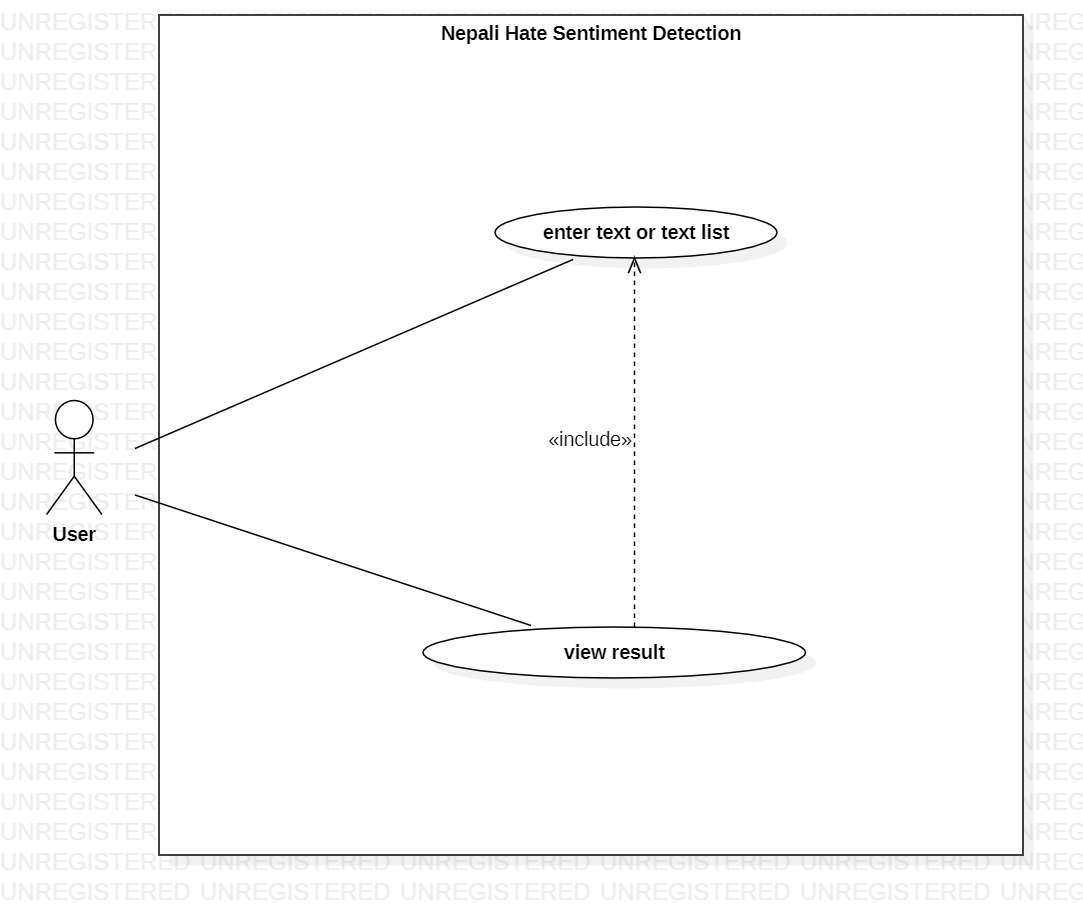
\includegraphics[scale=0.5]{images/usecase.png}
\caption{Usecase Diagram}
\end{figure}
\newpage
\subsubsection{DFD}
\begin{figure}[h]
\centering
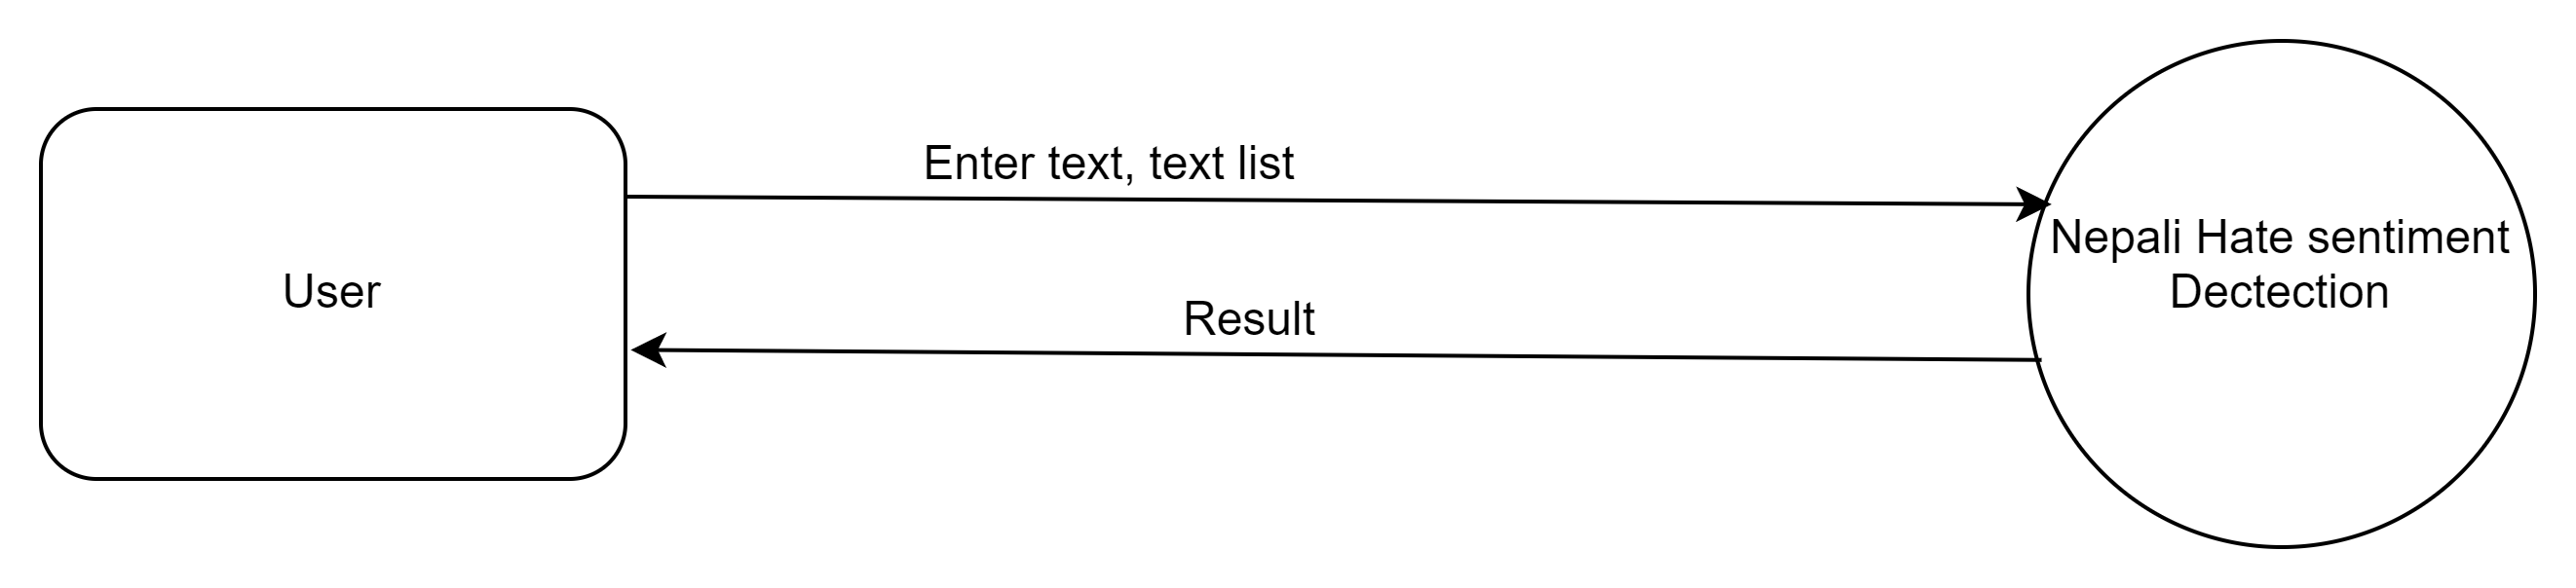
\includegraphics[scale=0.21]{images/dfd.png}
\caption{DFD diagram}
\end{figure}

%\subsection{Class Diagram}
%\subsection{Activity Diagram}

\chapter{Result and Discussions}
%\addcontentsline{toc}{chapter}{Result And Discussion}
\section{Works Completed}

The work till now encompasses experimentation on Classifiers and Encoders. The encoder used is Word2Vec, where the 300 dimensional vectors were used for classification through SVM with kernal "rbf". SVM was experimented on both unbalanced and balanced data instances. The balancing strategies constitutes of NCR, CNN and randomundersampling of majority class "GENERAL". Here, the class is first undersampled and experimented using NCR and CNN. These undersampled classes are then randomly undersampled to compliment minority class. The minority classes, on the otherhand, are experimented using SMOTE and ADASYN. The most favourable output was seen on CNN, Random under Sampler and SMOTE. The total count with such strategy resulted in 1200 instances, with Recall of 42.421\% and Precision of 35.544\%. This amounts to 35.56\% F1 score.
\begin{figure}[h]
\centering
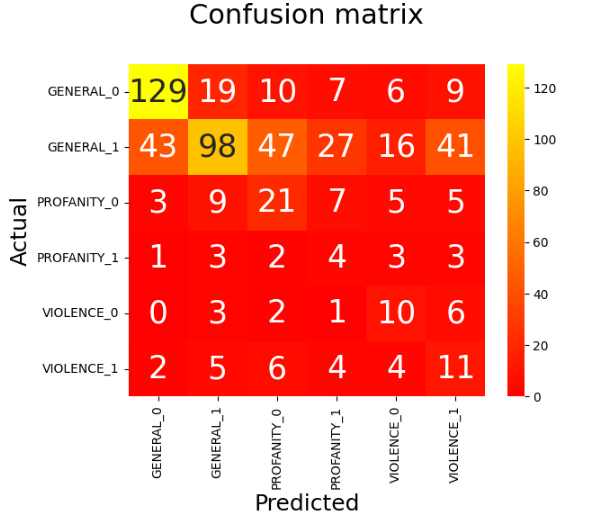
\includegraphics[scale=0.5]{images/confusion.png}
\caption{Confusion Matrix}
\end{figure}
 
\section{Works Remaining}
There are still experimentations to be done. To address class imbalance, we require a model that can handle minorities. Furthermore, Word2Vec might be struggling with capturing the semantics within the classes. Other encoders such as Fasttext, and GLOVE needs to be tested. Sentence level embedders such as NepBERTa and LASER could create better result when it comes to generating balanced embeddings.


%\section{Schedule}





\newpage
%Reference
\renewcommand{\bibname}{REFERENCES} % Change heading to References
\bibliographystyle{IEEEtran} % to use IEEE Format for referencing
\bibliography{majorReference} % specify the .bib file containing reference information 
\addcontentsline{toc}{chapter}{References} % to add references in TOC

%Comment this Chapter if you do not need to include Appendix.

%\addcontentsline{toc}{chapter}{Appendix}

% \begin{figure}[ht]
%     \centering
%     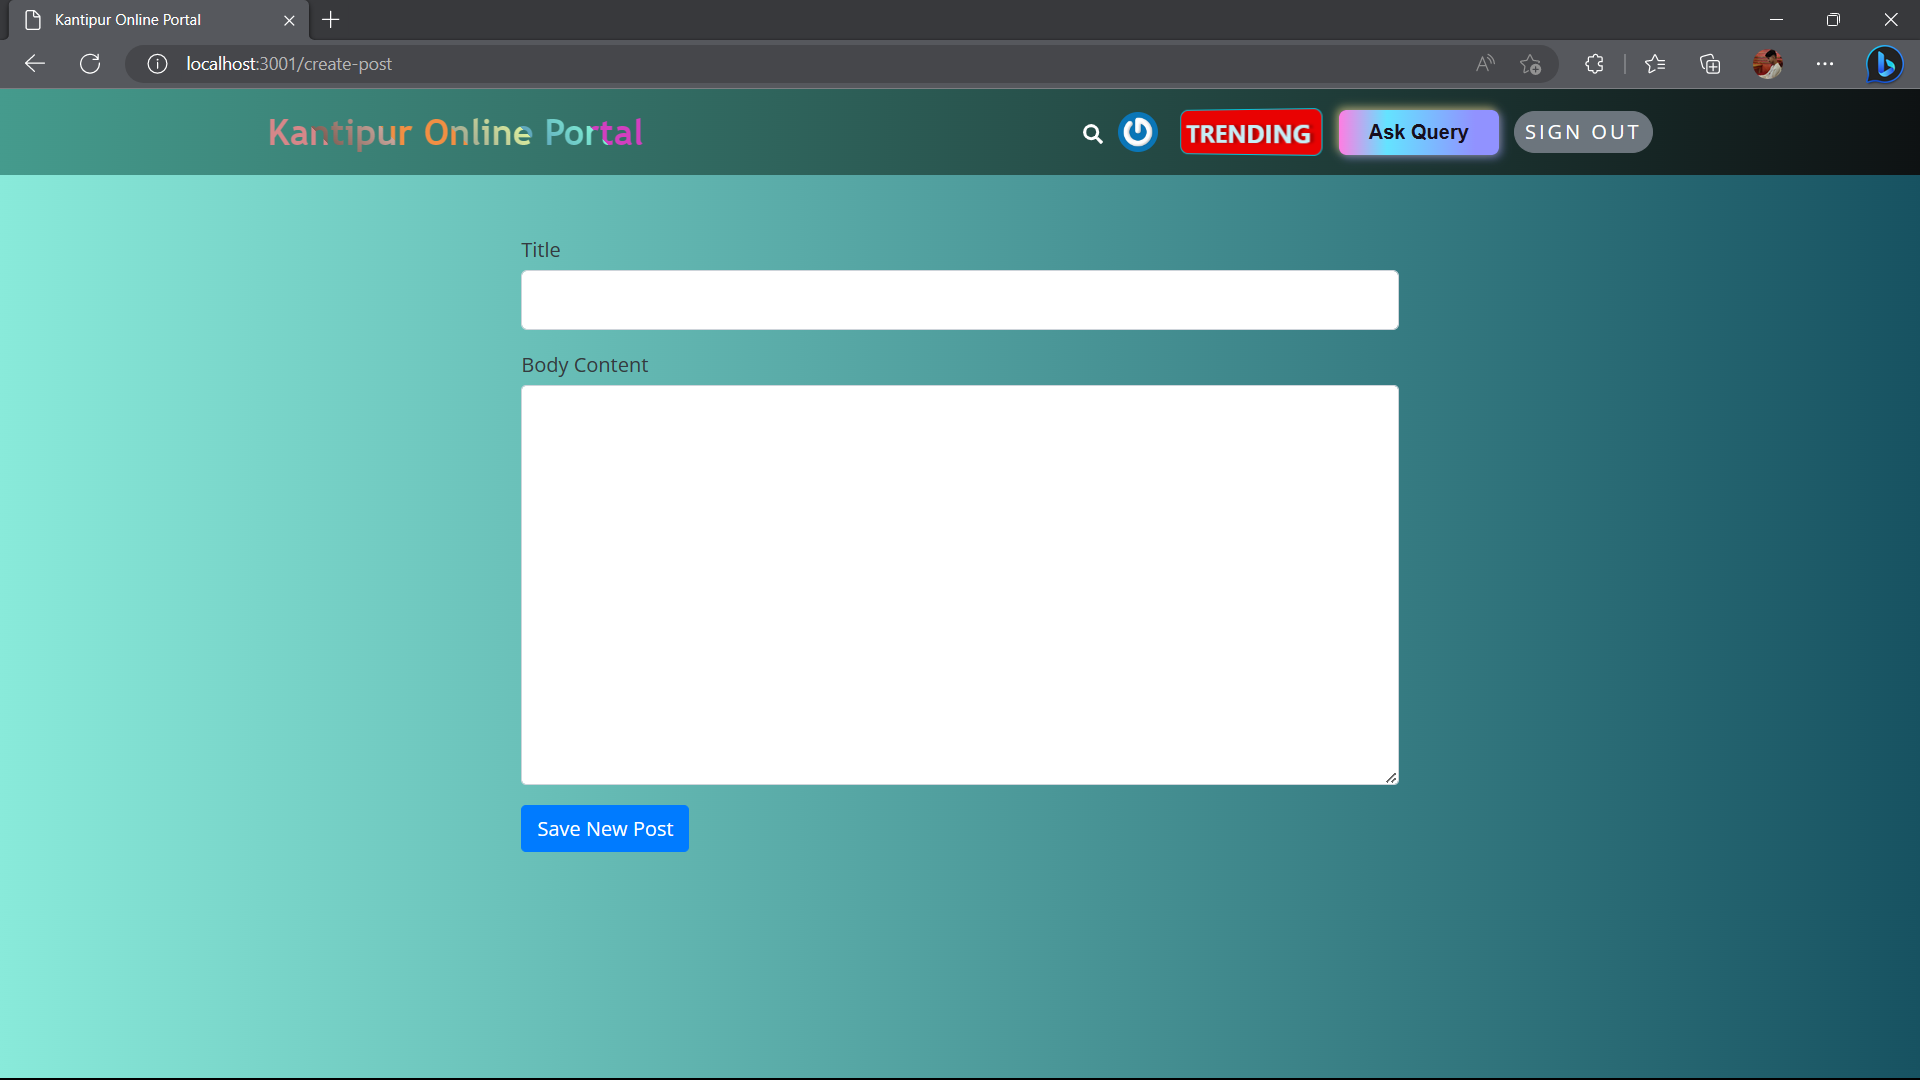
\includegraphics[scale=0.2]{pictures/2.png}
%    % \caption{Gantt Chart}
%    % \label{fig:my_label}
% \end{figure}

% \begin{figure}[ht]
%     \centering
%     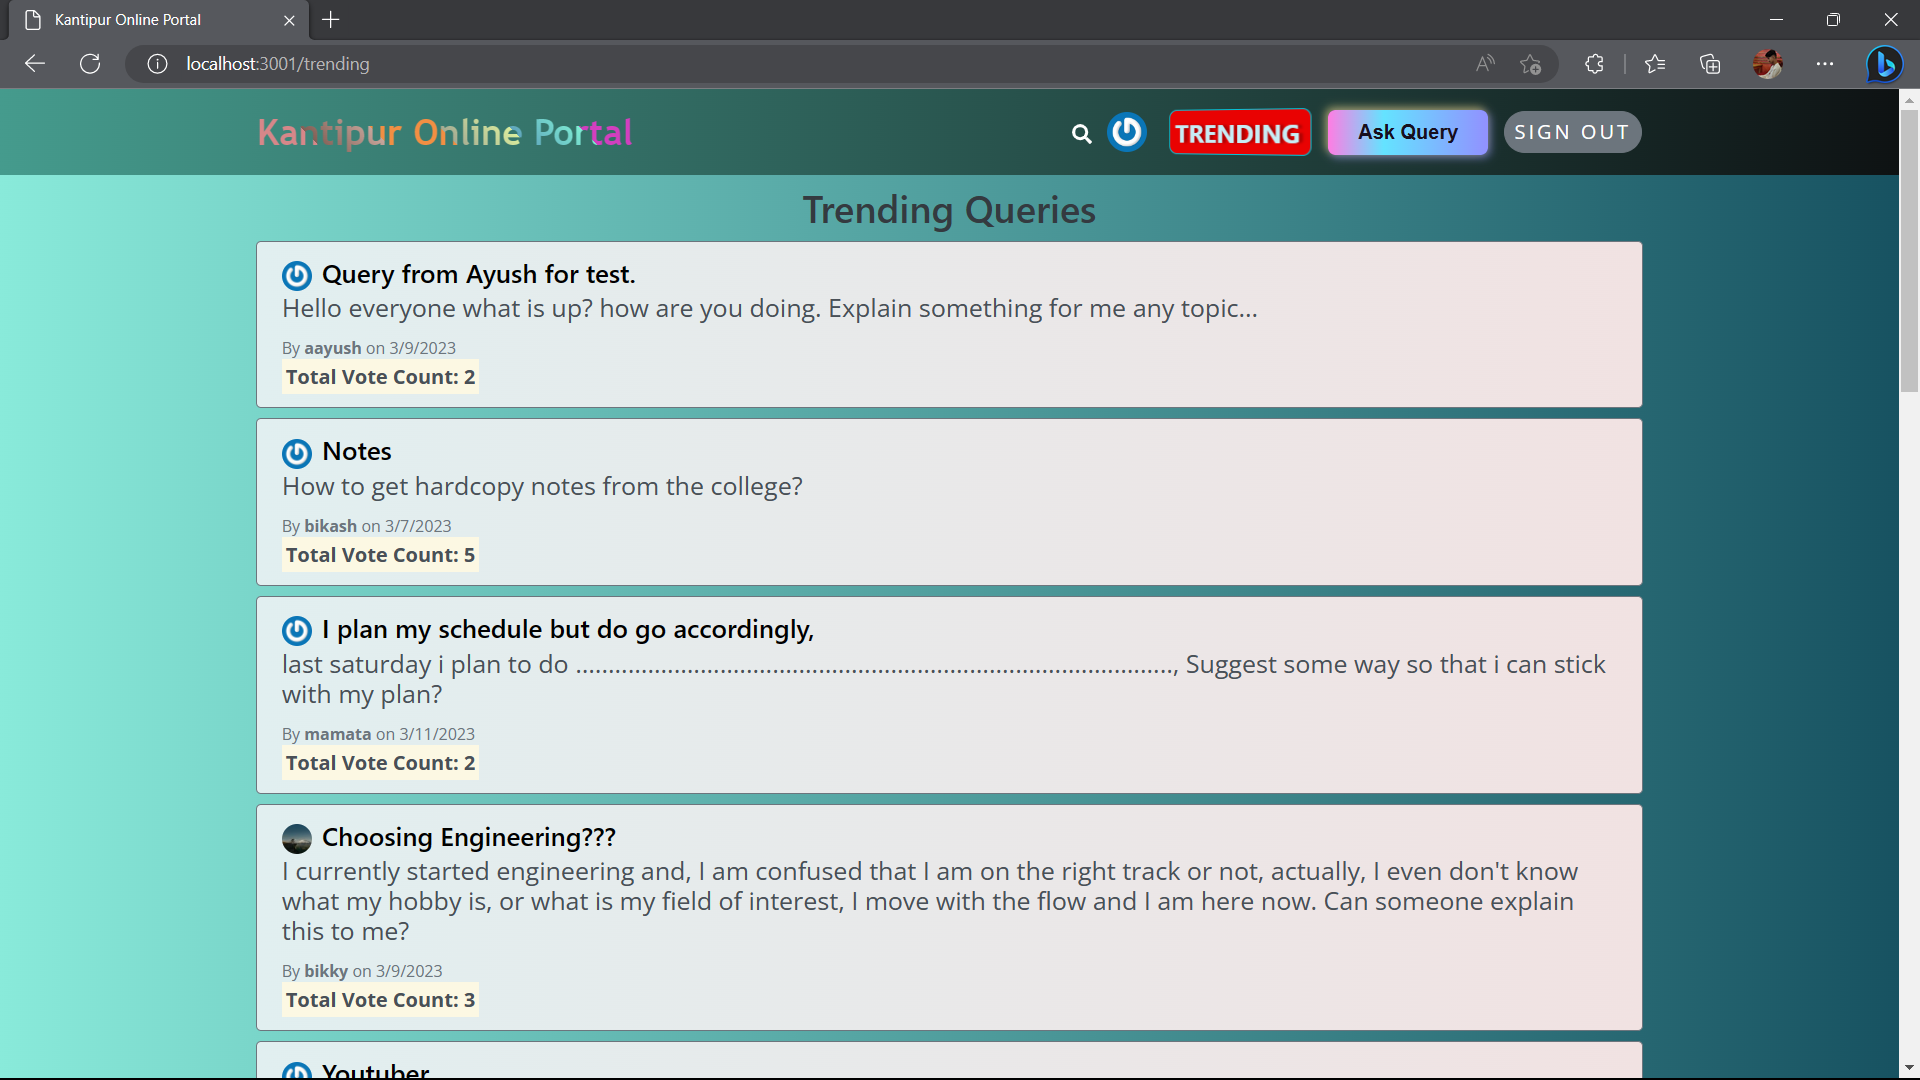
\includegraphics[scale=0.2]{pictures/3.png}
%    % \caption{Gantt Chart}
%    % \label{fig:my_label}
% \end{figure}

% \begin{figure}[ht]
%     \centering
%     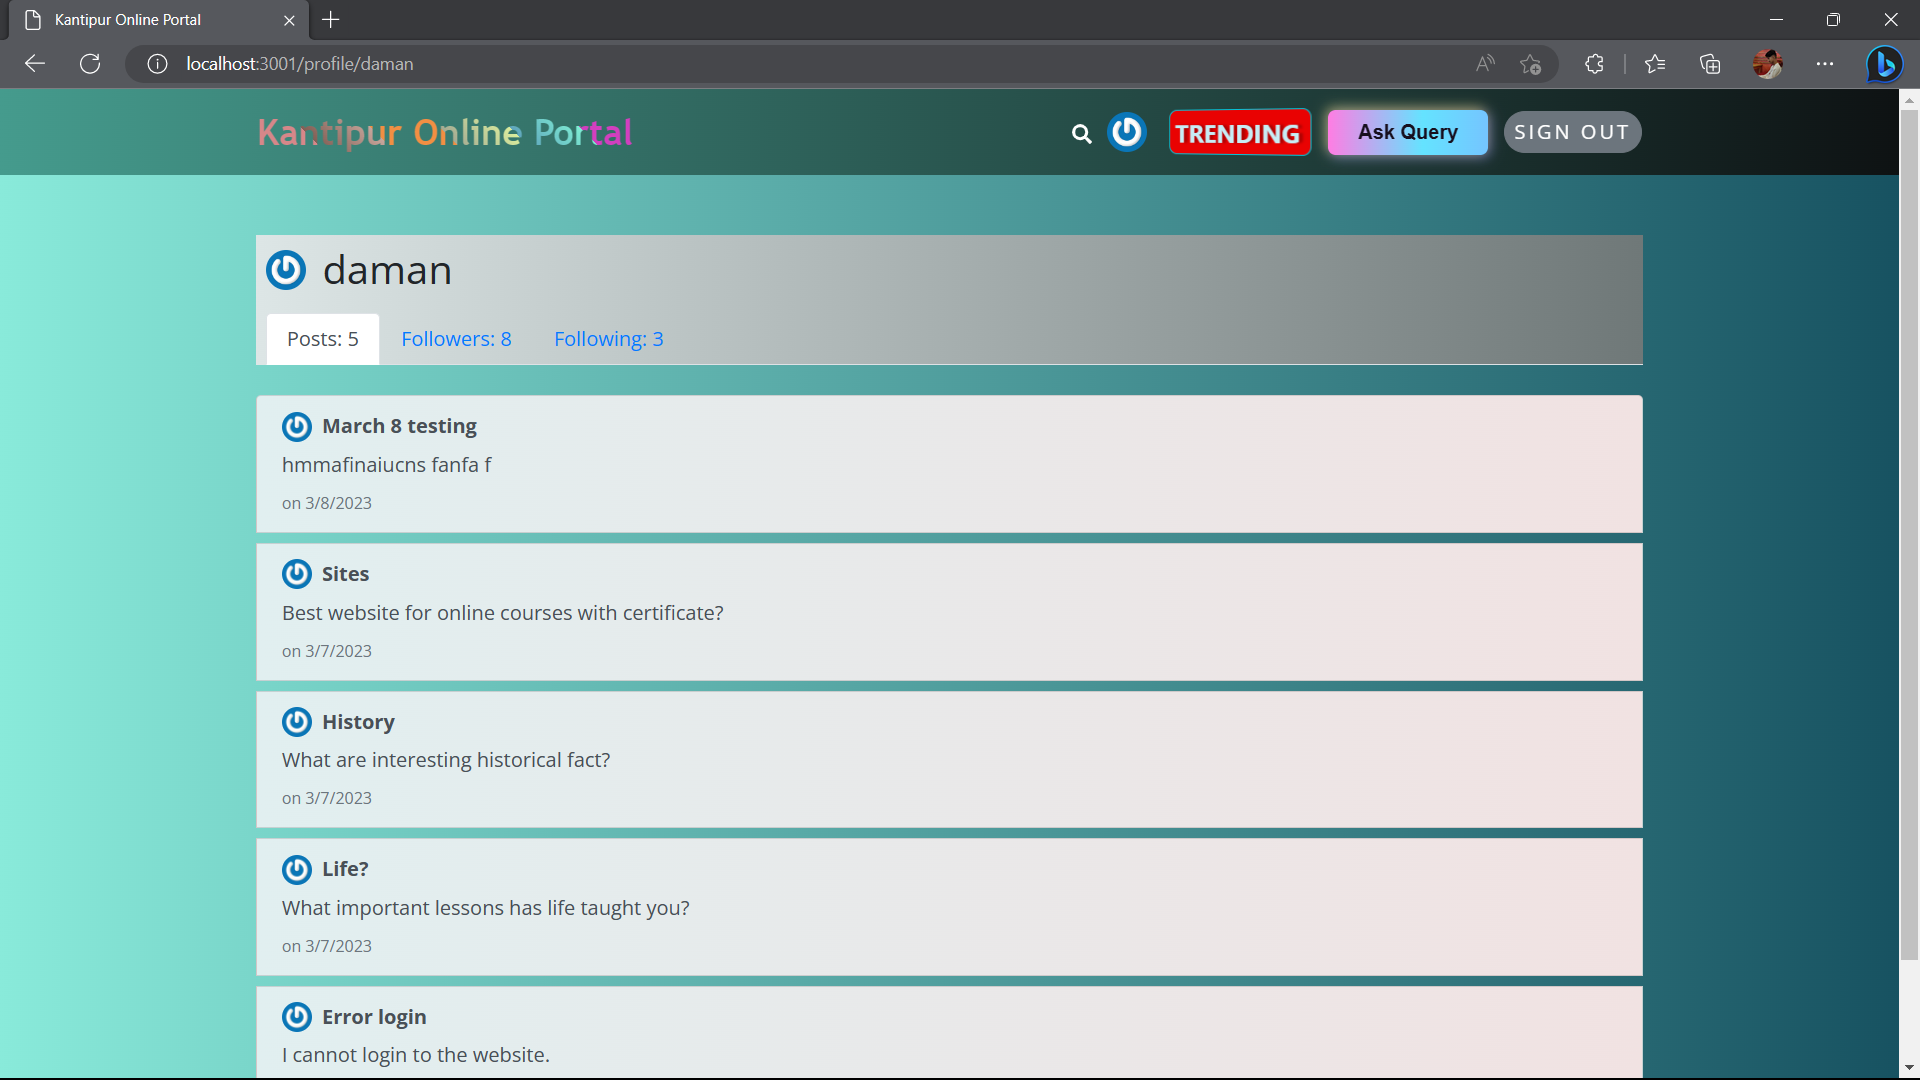
\includegraphics[scale=0.2]{pictures/4.png}
%    % \caption{Gantt Chart}
%    % \label{fig:my_label}
% \end{figure}

% \begin{figure}[ht]
%     \centering
%     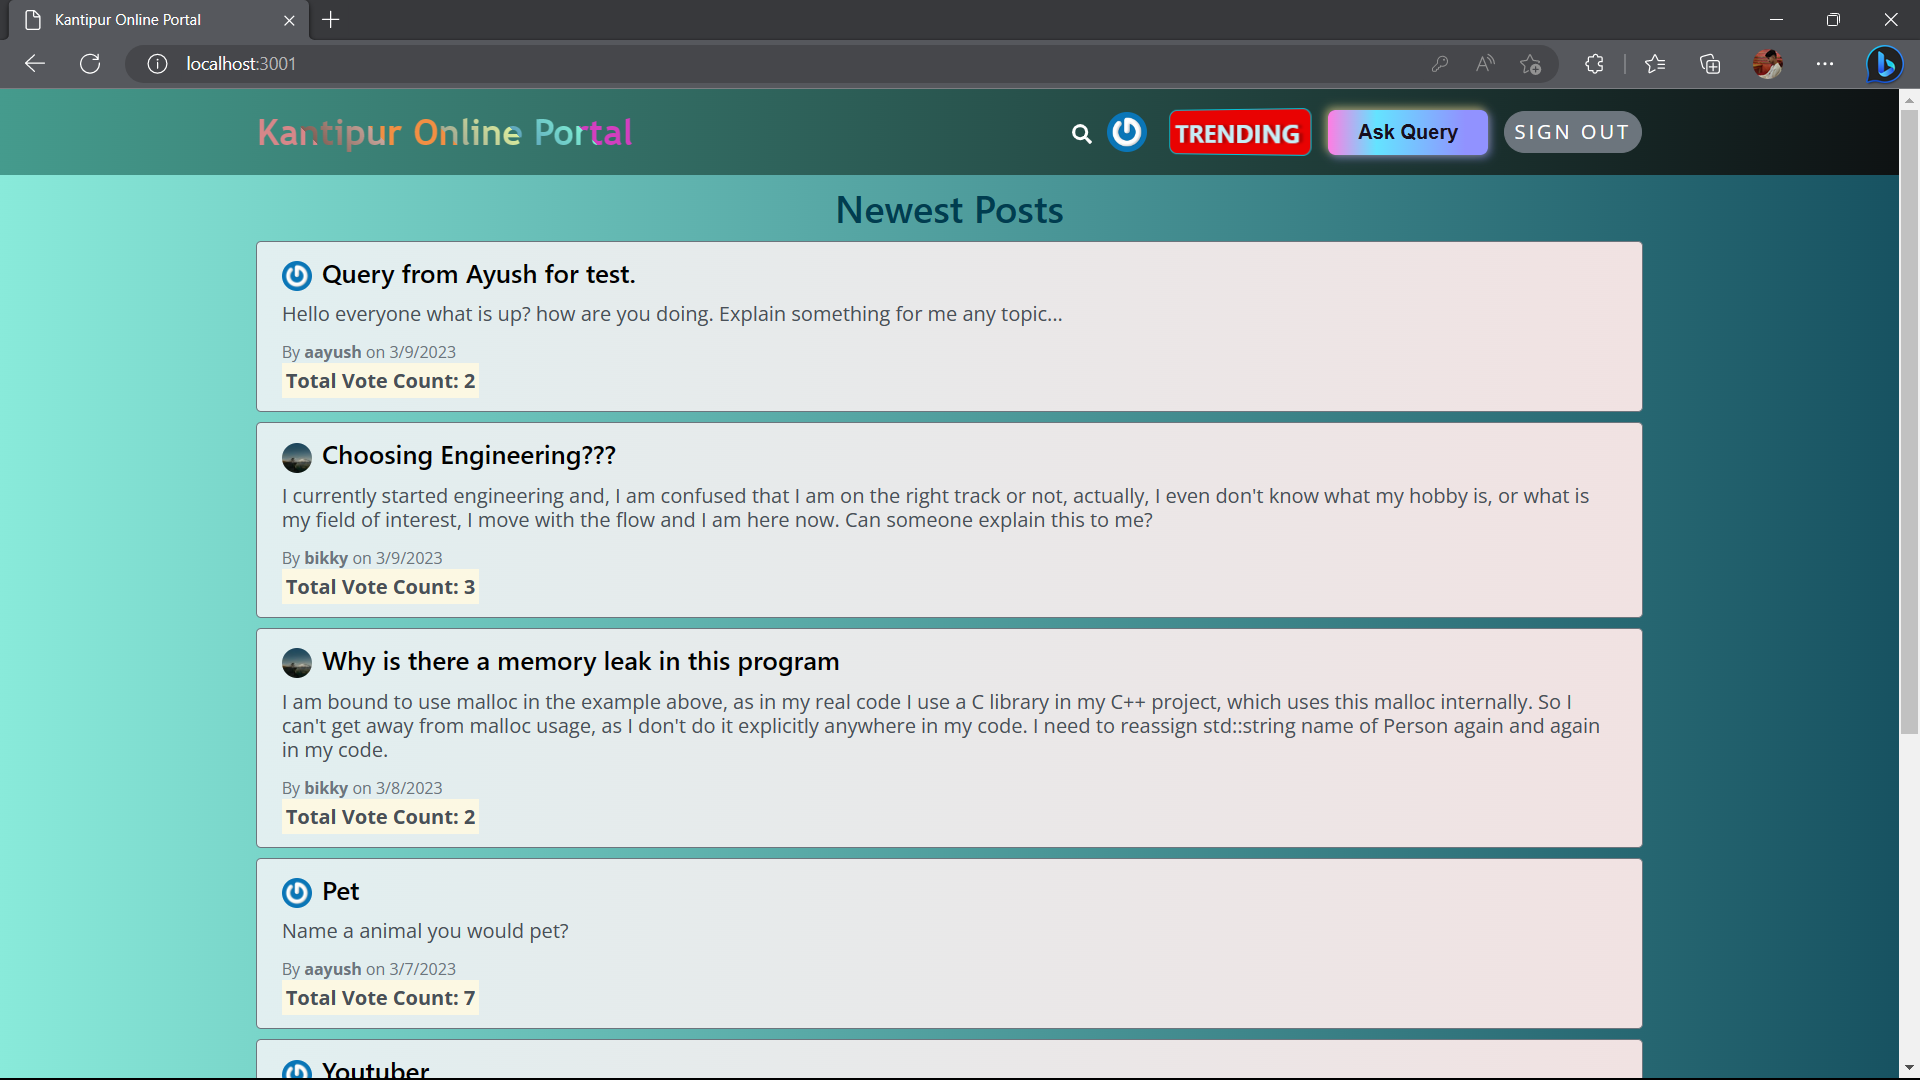
\includegraphics[scale=0.2]{pictures/5.png}
%    % \caption{Gantt Chart}
%    % \label{fig:my_label}
% \end{figure}
% \newpage
% \begin{figure}[ht]
%     \centering
%     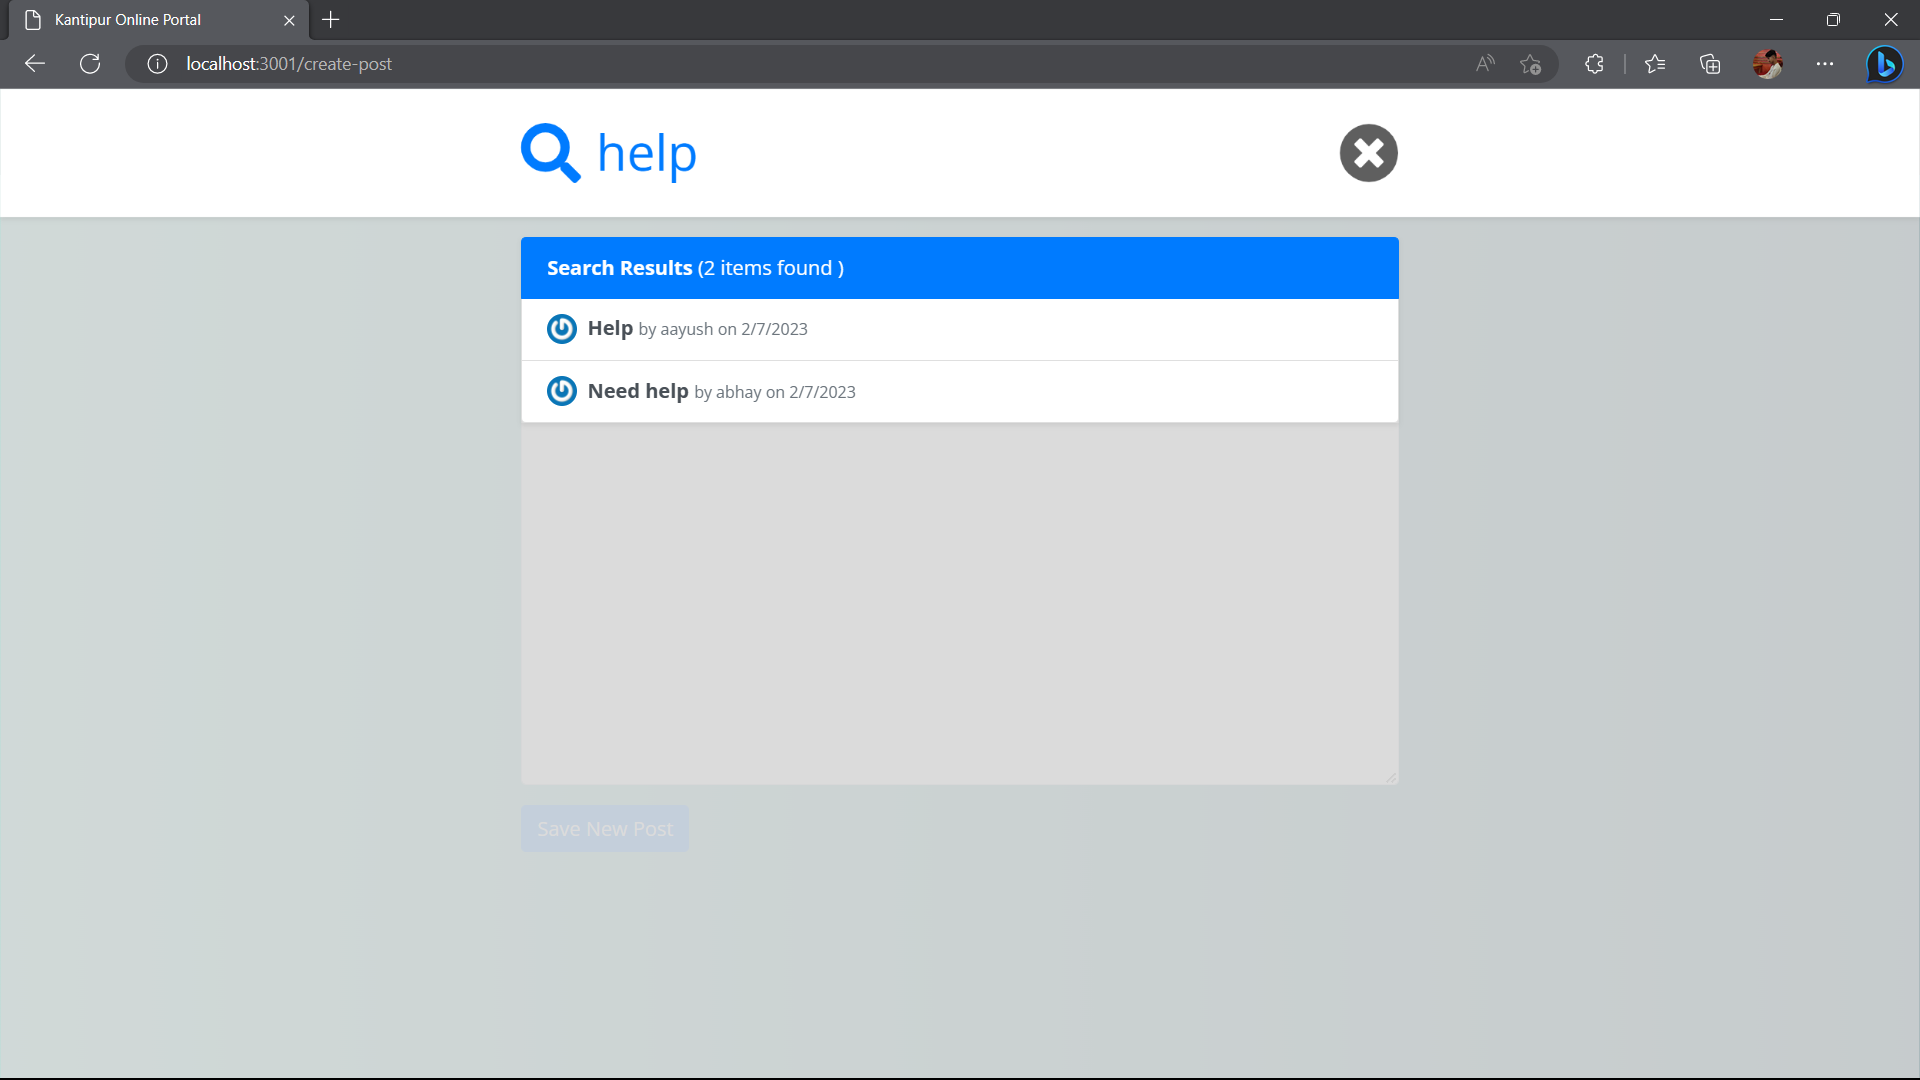
\includegraphics[scale=0.2]{pictures/6.png}
%    % \caption{Gantt Chart}
%    % \label{fig:my_label}
% \end{figure}

% \begin{figure}[ht]
%     \centering
%     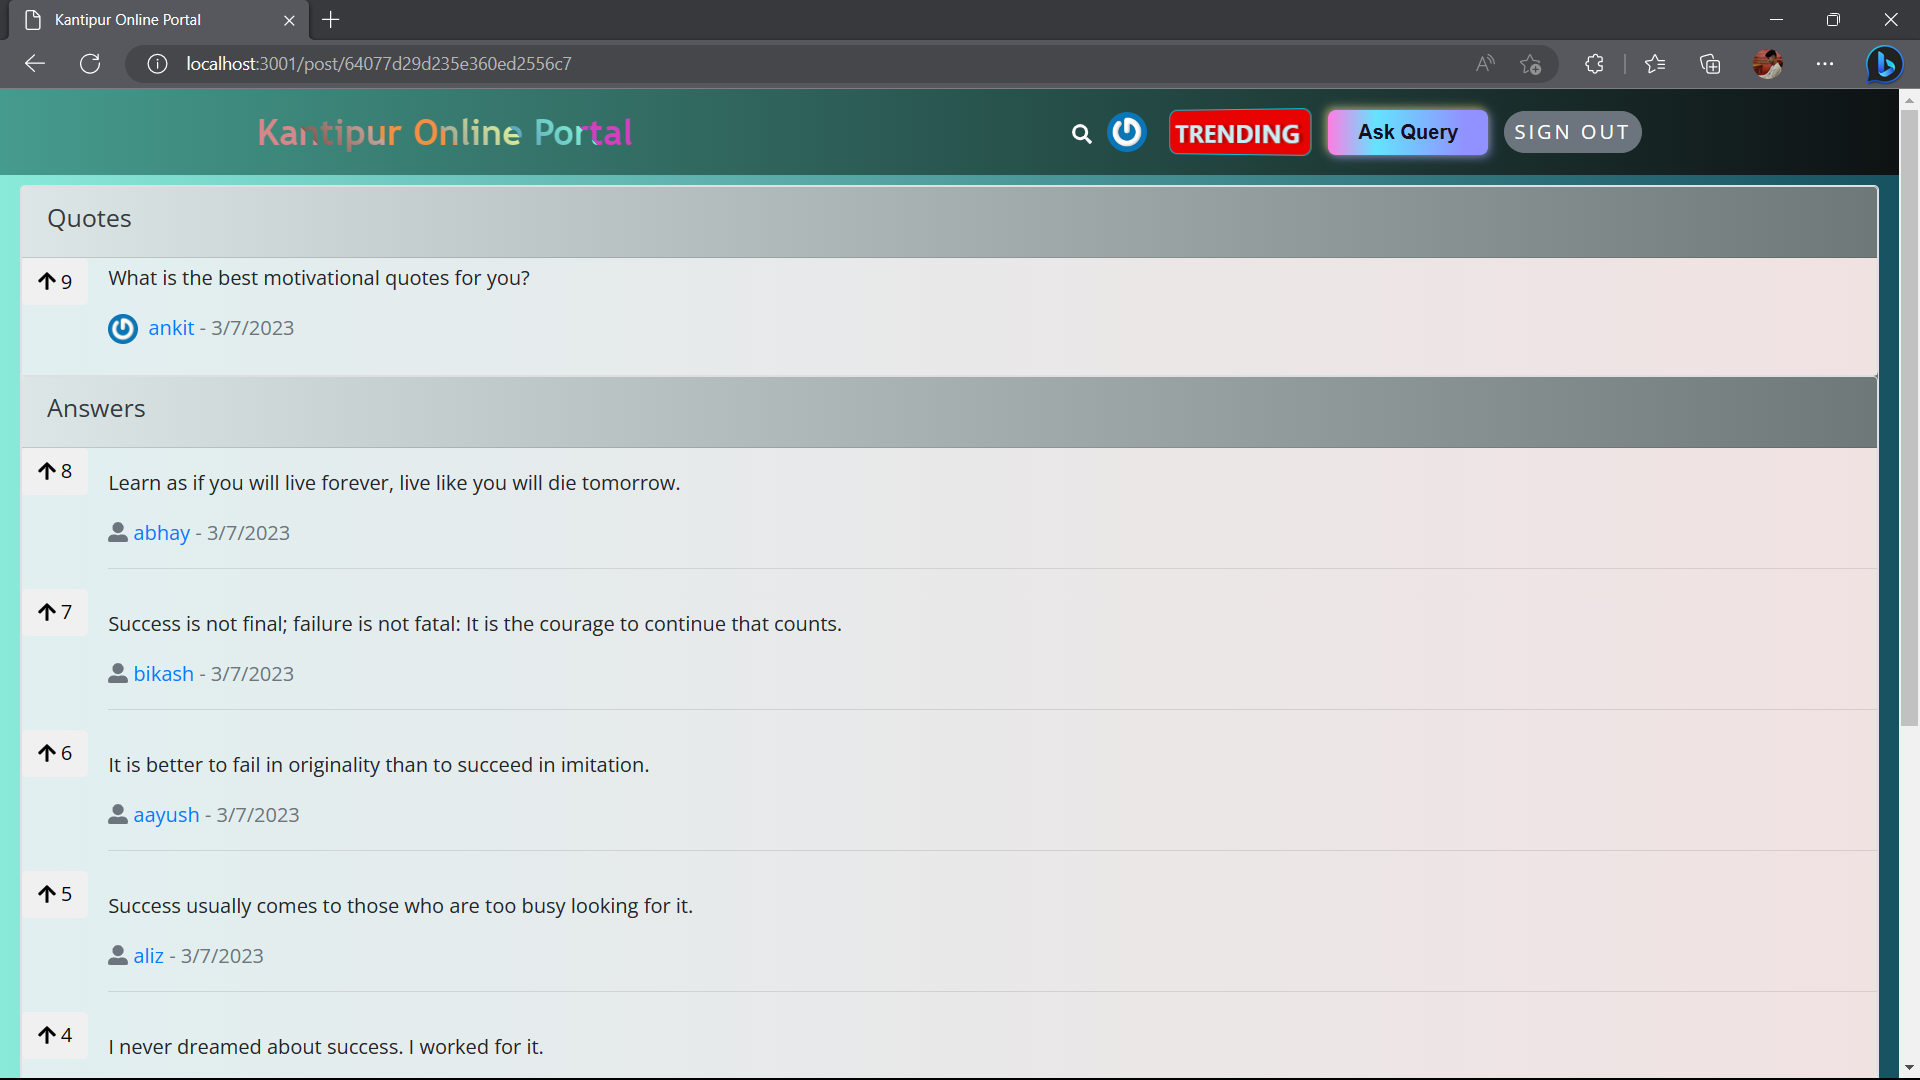
\includegraphics[scale=0.2]{pictures/7.png}
%    % \caption{Gantt Chart}
%    % \label{fig:my_label}
% \end{figure}

\nocite{goyal_2021}
\end{document}
